\documentclass[11pt]{article}
\usepackage[utf8]{inputenc}
\usepackage{algorithm}
\usepackage{amsmath}
\usepackage{graphicx}
\usepackage{caption}
\usepackage{subcaption}
\usepackage{mathtools}
\usepackage{amsfonts}
\usepackage{hyperref}
\usepackage{geometry}
\usepackage{multicol}
\usepackage{capt-of}
\usepackage{url}
\usepackage{chemmacros}
\usepackage{upgreek}
\usepackage{isomath}
\usepackage{cancel}
\usepackage{bm}
\usepackage[italian]{babel}
\geometry{a4paper, top=2.5cm, bottom=2.5cm, left=3cm, right=3cm, bindingoffset=5mm}
\usepackage[suftesi]{frontespizio}
\usepackage{siunitx}
\usepackage{float}
\usepackage{verbatim}

\title{Relazione di Laboratorio di Misure Nucleari\\ EFFETTO COMPTON }
\author{Damiano Algeri C.M. 967559\\damiano.algeri@studenti.unimi.it\\ \\ Nicolò Favagrossa C.M. 969124\\nicolo.favagrossa@studenti.unimi.it\\ \\ Michele Scattola C.M. 946576\\michele.scattola@studenti.unimi.it}
\date{\today\\A.A. 2023-2024}
\begin{document}
\maketitle
\newpage
\tableofcontents
\newpage
\section{Introduzione}
Lo scopo di questa relazione è esporre in maniera completa i processi logici e sperimentali riguardanti lo studio dell'effetto Compton. Quest'ultimo è uno dei possibili modi con cui i fotoni interagiscono con la materia. I protagonisti di questa esperienza sono due scintillatori inorganici: il primo è composto da cristalli di ioduro di sodio ($\ch{NaI}$) e il secondo da cristalli di bromuro di cerio ($\ch{CeBr_3}$). Gli obbiettivi principali sono: 
\begin{itemize}
    \item Verificare la relazione che descrive l'energia di un fotone Compton in funzione dell'angolo di scattering.
    \item Verificare la sezione d'urto espressa dall'equazione di Klein-Nishina.
\end{itemize}
%Dopo o nell'introduzione ci vorrebbe una parte in cui viene descritto l'esperimento altrimenti chi legge non capisce che cosa si è fatto e perchè
\section{Trattazione Teorica}
Prima di procedere all'analisi di questa esperienza è utile ricordare quale è la fisica coinvolta in questo esperimento.
\subsection{Attenuazione del fascio di particelle incidenti}
Se si prende un fascio di particelle incidenti su un mezzo il tasso totale di particelle diffuse si traduce in una diminuzione dell'intensità $I$ del fascio:
\begin{equation}
    \frac{dn}{dt} = -dI = I n_{T} dz \sigma
\end{equation}
da cui
\begin{equation}
    \frac{dI}{I(z)} = - n_{T} dz \sigma
\end{equation}
dove $n_{T}$ è la densità dei bersagli del mezzo, $dz$ è il suo spessore e $\sigma$ è la sezione d'urto totale. Se la diminuzione del numero di particelle non è trascurabile, come nel caso di questo esperimento, l'intensità varia con la profondità secondo la legge:
\begin{equation}
    I(z) = I_{0} e^{-\mu z}
\label{eq attenuazione fascio}
\end{equation}
dove $\mu = n_{T} \sigma$ è detto coefficiente di assorbimento che ha l'unità di misura dell'inverso di una lunghezza.
\subsection{Effetto Compton}
Lo scattering Compton è un fenomeno che descrive l'interazione tra una particella senza massa, un fotone, e una particella di massa non nulla che è considerata a riposo, un elettrone. L'assunzione fondamentale che l'elettrone bersaglio è a riposo è una buona approssimazione per atomi di elementi con basso $Z$ per i quali l'energia di legame dell'elettrone è minore dell'energia del fotone incidente.
Dunque il processo di scattering preso in considerazione è:
\begin{equation}
    \gamma + e^{-} \rightarrow \gamma + e^{-}
\end{equation}
La cinematica dello scattering Compton può essere facilmente derivata dalle leggi di conservazione dell'energia e del momento angolare in relatività ristretta. 
Per una particella con massa $m\neq{0}$ e quadrimpulso \textbf{p} = ($\frac{\gamma m c^{2}}{c}$, $p_{x}$, $p_{y}$, $p_{z}$) si può calcolare la massa invariante $\sqrt{\textbf{pp}}$ che in forma generale risulta:
\begin{equation}
    \textbf{pp} = \frac{E^{2}}{c^{2}} - p^{2} = m^{2} c^{2} \quad \text{oppure} \quad E^{2} - p^{2} c^{2} = m^{2} c^{4}
\label{massa invariante}
\end{equation}
E' chiaro che il processo di scattering avviene in un piano  geometrico che contiene tutti i momenti delle particelle coinvolte; assumiamo che questo piano sia il piano x-y trascurando la coordinata z. La situazione è rappresentata in Figura \ref{immagine scattering Compton}.
\begin{figure}[h]
    \centering
    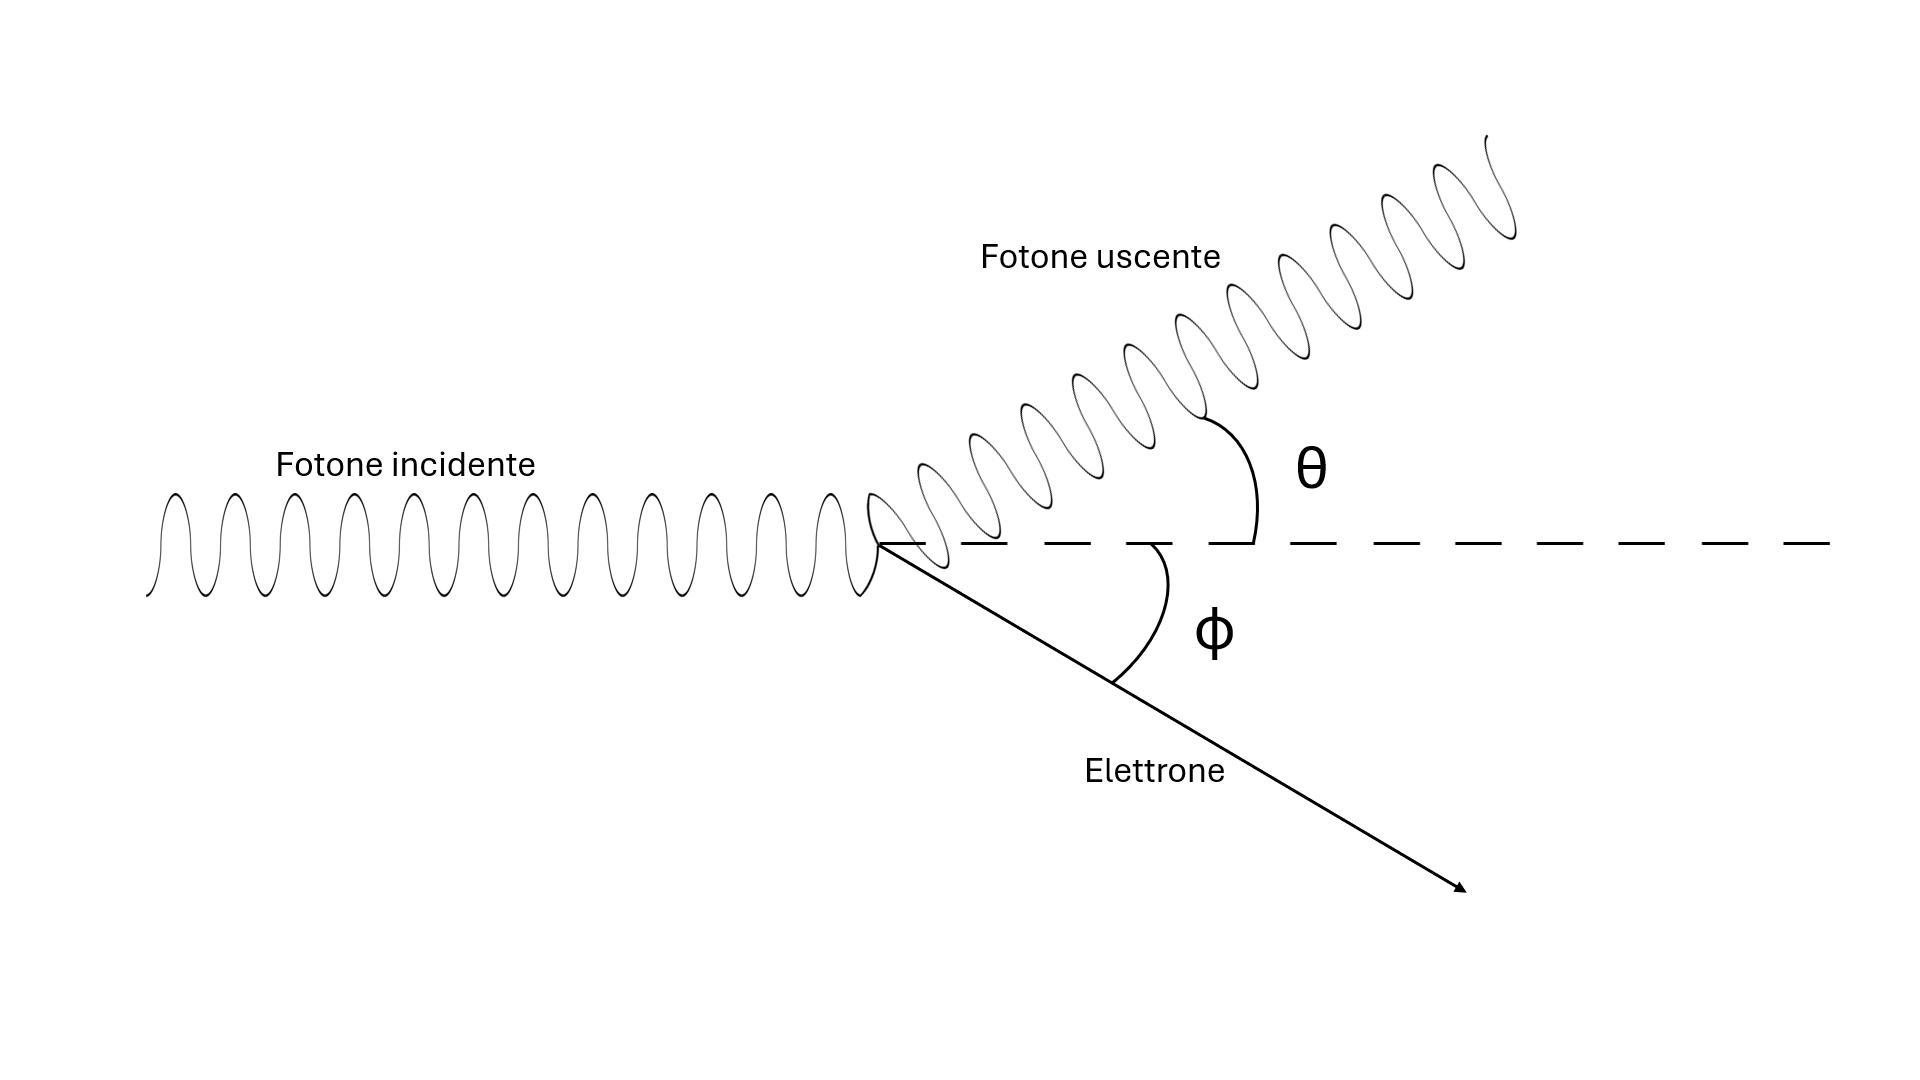
\includegraphics[width=0.85\textwidth]{Trattazione teorica/Scattering Compton.png}
    \caption{Scattering Compton nel piano x-y}
    \label{immagine scattering Compton}
\end{figure}

Chiamiamo $E_{0}$ l'energia del fotone incidente, $E_{1}$ l'energia del fotone uscente ed $E_{e}$ l'energia dell'elettrone e applichiamo la conservazione dell'energia e della quantità di moto usando le formule relativistiche:
\begin{equation}
    p_{x}: \quad \frac{E_{0}}{c} = \frac{E_{1}}{c} cos\theta + p\cdot cos\phi
\label{conservazione p asse x}
\end{equation}
\begin{equation}
    p_{y}: \quad \frac{E_{1}}{c} sin\theta - p\cdot sin\phi = 0
\label{conservazione p asse y}
\end{equation}
\begin{equation}
    E: \quad E_{0} + m c^{2} = E_{1} + E_{e}
\label{conservazione energia}
\end{equation}
dove $p$ è il modulo della quantità di moto dell'elettrone, $m$ è la massa dell'elttrone e $\theta$ e $\phi$ sono gli angoli che le particelle uscenti formano con la direzione del fotone incidente.
Dalla conservazione della quantità di moto (eq. \eqref{conservazione p asse x} e \eqref{conservazione p asse y}) si ottiene:
\begin{equation}
    E_{0} - E_{1} \cdot cos\theta = pc\cdot cos\phi
\end{equation}
\begin{equation}
    E_{1} \cdot sin\theta = pc\cdot sin\phi
\end{equation}
Elevando al quadrato e sommando:
\begin{equation}
    E_{1}^{2} \cdot sin^{2}\theta + (E_{0} - E_{1} \cdot cos\theta)^{2} = p^{2}c^{2} (sin^{2}\phi + cos^{2}\phi)
\end{equation}
da cui:
\begin{equation}
    E_{1}^{2} + E_{0}^{2} - 2 E_{0} E_{1} cos\theta = p^{2}c^{2}
\label{cons p al quadrato e sommate}
\end{equation}
Dalla conservazione dell'energia (eq. \eqref{conservazione energia}) si può esplicitare $E_{e}$:
\begin{equation}
    E_{e} = E_{0} + m c^{2} - E_{1}
\label{Ee esplicitata}
\end{equation}
mentre dall'eq. \eqref{massa invariante} applicata all'elettrone si ricava $p^{2}c^{2} = E_{e}^{2} - m^{2} c^{4}$. Mettendo insieme queste due si ottiene:
\begin{equation}
    p^{2}c^{2} = (E_{0} - E_{1} + m c^{2})^{2} - m^{2} c^{4} = (E_{0} - E_{1})^{2} + 2 m c^{2}(E_{0} - E_{1})
\end{equation}
che sostituita nella \eqref{cons p al quadrato e sommate} porta a:
\begin{equation}
    E_{0}^{2} + E_{1}^{2} - 2E_{0}E_{1} + 2 m c^{2}(E_{0} - E_{1}) = E_{1}^{2} + E_{0}^{2} - 2 E_{0} E_{1} cos\theta
\end{equation}
Esplicitando l'energia del fotone scatterato si ha:
\begin{equation}
    E_{1} = \frac{E_{0}}{1 + \frac{E_{0}}{m_{e}c^{2}}(1-cos\theta)}
    \label{energia fotone uscente}
\end{equation}
Come si può notare l'energia del fotone uscente dipende strettamente dall'angolo di scattering.
\subsection{Sezione d'urto e formula di Klein-Nishina}
Se assumiamo che il centro di scattering tra le particelle sia un nucleo inizialmente fermo avremo che la densità dei centri di scattering nel bersaglio è data da:
\begin{equation}
    N = \rho \frac{N_{A}}{M}
\end{equation}
dove $\rho$ è la densità del bersaglio, $M$ la sua massa atomica e $N_{A}$ il numero di Avogadro. Nel nostro caso, dato che i fotoni interagiscono con gli elettroni del nucleo bersaglio, $N$ va moltiplicato per $Z$. Il numero di particelle deviate $N_{S}$ è proporzionale al numero di particelle incidenti $N_{i}$, al numero di centri di diffusione incontrati e alla sezione d'urto dei singoli centri, dunque:
\begin{equation}
    N_{S} = N_{i} N dx \sigma = N_{i} \rho \frac{N_{A}}{M} dx \sigma
\label{eq particelle scatterate}
\end{equation}
Nel nostro esperimento non vogliamo sapere solo quante particelle vengono deviate, ma vogliamo sapere anche a quale angolo; parliamo quindi di sezione d'urto differenziale. Perché abbiano senso le misure occorre normalizzare i conteggi rispetto all'angolo solido coperto dal rivelatore, pertanto, anche grazie all'eq \eqref{eq particelle scatterate}, si ottiene:
\begin{equation}
    \frac{d\sigma}{d\Omega} = \frac{1}{\Delta\Omega} \frac{N_{S}}{N_{i}} \frac{M}{N_{A} \rho dx}
\label{eq sezione d'urto conteggi}
\end{equation}
Nell'analisi dei dati di questo esperimento ci siamo serviti anche della formula di Klein-Nishina che ci permette di calcolare la sezione d'urto in funzione dell'energia del fotone scatterato:
\begin{equation}
    \frac{d\sigma}{d\Omega} = \frac{1}{2} r_{e}^{2} \left(\frac{k_{1}}{k_{0}}\right)^{2} \left(\frac{k_{1}}{k_{0}} + \frac{k_{0}}{k_{1}} - \sin^{2}{\theta}\right)
\end{equation}
dove
\begin{equation}
    r_{e} = \frac{e^{2}}{4 \pi \epsilon_{0} m_{e} c^{2}} \quad k_{0} = \frac{E_{0}}{m_{e} c^{2}} \quad k_{1} = \frac{E_{1}}{m_{e} c^{2}}
\end{equation}
Nel nostro caso $k_{0} = 1$ dunque:
\begin{equation}
    \frac{d\sigma}{d\Omega} = \frac{1}{2} r_{e}^{2} k_{1}^{2} \left(k_{1} + \frac{1}{k_{1}} - \sin^{2}{\theta}\right)
\label{eq sezione d'urto Klein-Nishina}    
\end{equation}


\newpage
\section{Materiali e Strumentazione}
La tecnica sperimentale impiegata per analizzare l'effetto Compton prevede di far incidere un fascio di fotoni, emesso da una sorgente radioattiva, su un bersaglio che serve da scatteratore. I fotoni prodotti e i fotoni scatterati sono rilevati attraverso due scintillatori. Il primo funge da gate e conteggio, il secondo, posto a vari angoli rispetto ai fotoni incidenti serve da spettrometro.
\subsection{Sorgente}
I due fotoni sono prodotti attraverso il decadimento $\beta^+$ della sorgente radioattiva $\ch{^{22}Na}$\footnote{Tutti i dati sono presi da: \url{https://nds.iaea.org/relnsd/vcharthtml/VChartHTML.html}}. ($\mathrm{BR}=89.90\,\%$, $t_{1/2}=2.6\,\mathrm{yr}$). 
\begin{equation}
    \ch{^{22}Na}\,\to\,\ch{^{22}Ne^*}+e^++\nu_e
\end{equation}
 %IMMAGINE sodiodecay
\begin{figure}[htp!]
  \centering
  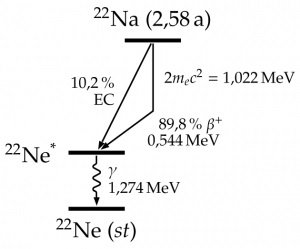
\includegraphics[scale=0.6]{Strumenti/sodiodecay.jpg} 
  \caption{Qui è possibile visualizzare in maniera schematica le due modalità di decadimento del $\ch{^{22}Na}$ e il diseccitamento elettromagnetico del $\ch{^{22}Ne^*}$}
\end{figure}
%va ridisegnato lo schema in quanto dal sito: https://nds.iaea.org/relnsd/vcharthtml/VChartHTML.html sono presenti dati leggermente diversi
La sorgente è sigillata all'interno di un involucro che induce tutti i positroni all'annichilazione con gli elettroni presenti nel materiale. La radiazione risultante è l'emissione di due $\gamma$ back to back con un'energia fissa di $511\,\unit{\kilo\electronvolt}$.
\begin{equation}
    e^++e^-\,\to\,2\gamma\,(511\,\unit{\kilo\electronvolt})
\end{equation}
La diseccitazione elettromagnetica del nucleo di $\ch{^{22}Ne^*}$ avviene in $t=3.6\,\unit{ps}$ con l'emissione di un $\gamma$ di energia $1274\,\unit{keV}$.
\begin{equation}
    \ch{^{22}Ne^*}\,\to\,\ch{^{22}Ne}+\gamma\,(1274\,\unit{keV})
\end{equation}
Oltre al decadimento $\beta^+$ è anche possibile la cattura elettronica con: $\mathrm{BR}=10.04\,\%$
\begin{equation}
    \ch{^{22}Na}+e^-\,\to\,\ch{^{22}Ne^*}+\nu_e
\end{equation}
L'attività della sorgente corrisponde a: $A=100,\unit{kBq}$.


Ricapitolando per ogni decadimento $\beta$ vengono emessi tre fotoni: i due provenienti dall'annichilazione di elettrone e positrone sono correlati in energie e direzione mentre il terzo è emesso in contemporanea ma in direzione casuale. L'emissione di due fotoni in direzione opposta alla stessa energia è una caratteristica fondamentale che rende possibile l'esecuzione della misura di coincidenza temporale tramite i due rivelatori: il rivelatore che svolge la funzione di spettrometro (indicato con A) e il secondo rilevatore (indicato con B) posizionato in direzione opposta allo scatteratore. 
\subsection{Rivelatori}
Il setup sperimentale è costituito da due scintillatori cilindrici inorganici. Il primo è uno scintillatore al cristallo di bromuro di cerio $\ch{CeBr_3}$ (usato come spettrometro e indicato con A), mentre il secondo è ai cristalli di ioduro di sodio $\ch{NaI}$ (usato come gate e indicato con B). Per quanto riguarda il secondo scintillatore è stato usato un drogante al tallio $\ch{Tl}$ il quale aggiunge livelli energetici ammessi all'interno della banda di energia proibita. Questi livelli in più hanno una doppia funzione: la prima è facilitare la ricombinazione elettrone-lacuna e la seconda è ridurre l'energia dell'emissione di luce rispetto a quella della bandgap. Entrambi gli scintillatori sono accoppiati a un fotomoltiplicatore.

Nella seguente tabella è possibile osservare le principali caratteristiche dei due scintillatori utilizzati:
\begin{table}[H]
    \centering
    \begin{tabular}{|c|c|c|c|c|c|}
    \hline
       Scintillatore  & $\rho$ $[\unit{g}/\unit{cm^3}]$ & $\lambda$ $[\unit{nm}]$ & $\tau$ $[\unit{ns}]$ & L.Y. $[\gamma/\unit{keV}]$ & $\Delta E/E$ $[\%]$ \\
    \hline
    \hline
    $\ch{CeBr_3}$ & $5.2$ & $380$ & $18$ & $45$ & $5$ \\
    \hline
    $\ch{NaI}:\ch{Tl}$ & $3.7$ & $415$ & $230$ & $38$ & $6$ \\
    \hline
    \end{tabular}
    \caption{Sono presentati i vari valori indicativi delle caratteristiche principali dei due scintillatori utilizati, senza errori corrispondenti.}
    \label{tab:scintillatori}
\end{table}

\subsection{Elettronica nucleare}\label{Elettronica nucleare}
Per riuscire a misurare e digitalizzare il segnale viene usata una catena elettronica divisa in diversi stadi. Lo schema dell'elettronica è presente nella figurag(\ref{fig:elettronica}). Quando la radiazione ionizzante interagisce con lo scintillatore, essa perde energia tramite processi come l'effetto fotoelettrico e l'effetto Compton. Gli elettroni generati da queste interazioni ionizzano il cristallo e, durante la ricombinazione con le lacune, vengono emessi numerosi fotoni, che ricadono generalmente nella banda del visibile. La quantità di fotoni emessi è proporzionale all'energia rilasciata dalla radiazione ionizzante. Una proprietà fondamentale dello scintillatore è il rendimento luminoso ($L_y$), espresso in termini di fotoni per $\unit{\kilo\electronvolt}$ ($\gamma/\unit{\kilo\electronvolt}$). 

Successivamente, i fotoni a bassa energia colpiscono il fotomoltiplicatore collegato al rivelatore. Questo processo estrae i primi elettroni dal fotocatodo, con una determinata efficienza quantica. Gli elettroni generati vengono quindi accelerati da un campo elettrico e colpiscono il primo elettrodo, chiamato dinodo, avviando una cascata di produzione di ulteriori elettroni. Infine, il segnale viene raccolto dall'anodo. Il segnale in uscita dipende dalla tensione di alimentazione del fototubo. 

Il segnale, trasportato attraverso cavi di tipo BNC, viene poi amplificato elettronicamente da uno stadio di preamplificazione in cui è importante fare attenzione al rapporto tra segnale e rumore. Il segnale amplificato viene trasferito in un amplificatore formatore necessario a dare la forma adatta per essere misurato massimizzando il rapporto segnale rumore. L'altezza dell'impulso viene misurata da un analizzatore multicanale (MCA). Questo dispositivo elettronico campiona il segnale al suo valore massimo e crea un istogramma, che mostra la distribuzione del numero di segnali campionati nei vari intervalli di ampiezza. Ogni canale dell'MCA corrisponde a un intervallo di tensione. Il campionamento del segnale avviene solo quando l'ampiezza del segnale in ingresso supera una soglia regolabile.

Per lo scopo di questo esperimento il rivelatore A è messo in coincidenza con il rivelatore B che funziona da Gate. Questo significa che quando dal software MAESTRO viene impostata la funzione di coincidenza gli unici segnali che vengono digitalizzati sono quelli in coincidenza con l'apertura del gate. Una descrizione più approfondita verrà fatta nella sezione dedicata alla calibrazione (\ref{Sez calibrazione}).
 %IMMAGINE eletronic_chain
\begin{figure}[htp!]
  \centering
  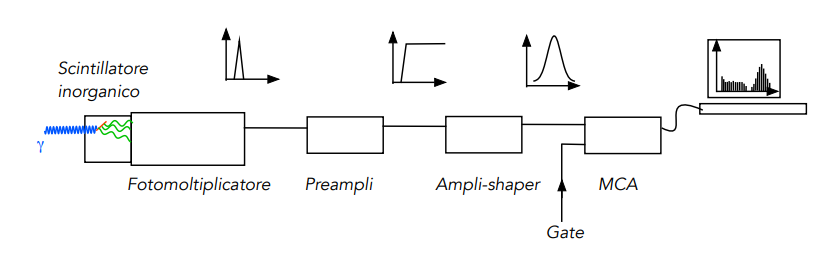
\includegraphics[scale=0.7]{Strumenti/electronic_chain.png} 
  \caption{In questa immagine è possibile visualizzare in maniera schematica la catena elettronica che caratterizza l'esperimento seguendo il segnale dal rivelatore alla sua digitalizzazione.}
  \label{fig:elettronica}
\end{figure}
\section{Apparato Sperimentale}
L'apparato sperimentale, visibile schematicamente nella fig. \ref{fig:apparato_sperimentale} è quindi costituito da:
\begin{itemize}
    \item Uno scintillatore inorganico cilindrico ai cristalli di $\ch{NaI} (\ch{Tl})$ accoppiato ad un fotomoltiplicatore;
    \item uno scintillatore inorganico cilindrico ai cristalli di $\ch{BeCr_3}$ accoppiato ad un fotomoltiplicatore,
    \item alimentatore ad alta tensione BERTAN Associates Model 313A che alimenta il fotomoltiplicatore accoppiato al rivelatore A,
    \item alimentatore ad alta tensione ORTEC 556 che alimenta il fotomoltiplicatore accoppiato al rivelatore B;
    \item due preamplitifacori SILENA che preamplificano il segnale uscente dai fotomoltiplicatori;
    \item amplificatore ORTEC AMP\&SCA 490A utilizzato per selezionare la finestra sul picco fotoelettrico per il gate;
    \item amplificatore ORTEC RESEARCH AMPLIFIER 450 utilizzato per formare il segnale da digitalizzare;
    \item un Multi-channel-Analyzer (MCA) inserito come scheda di espansione del PC utilizzato per acquisire lo spettro tramite il software MAESTRO;
    \item oscilloscopio Tektronix TDS 1002;
    \item modulo OPEN\_NIM che permette di effettuare i conteggi. 
\end{itemize}
 %IMMAGINE apparato_sperimentale
\begin{figure}[htp!]
  \centering
  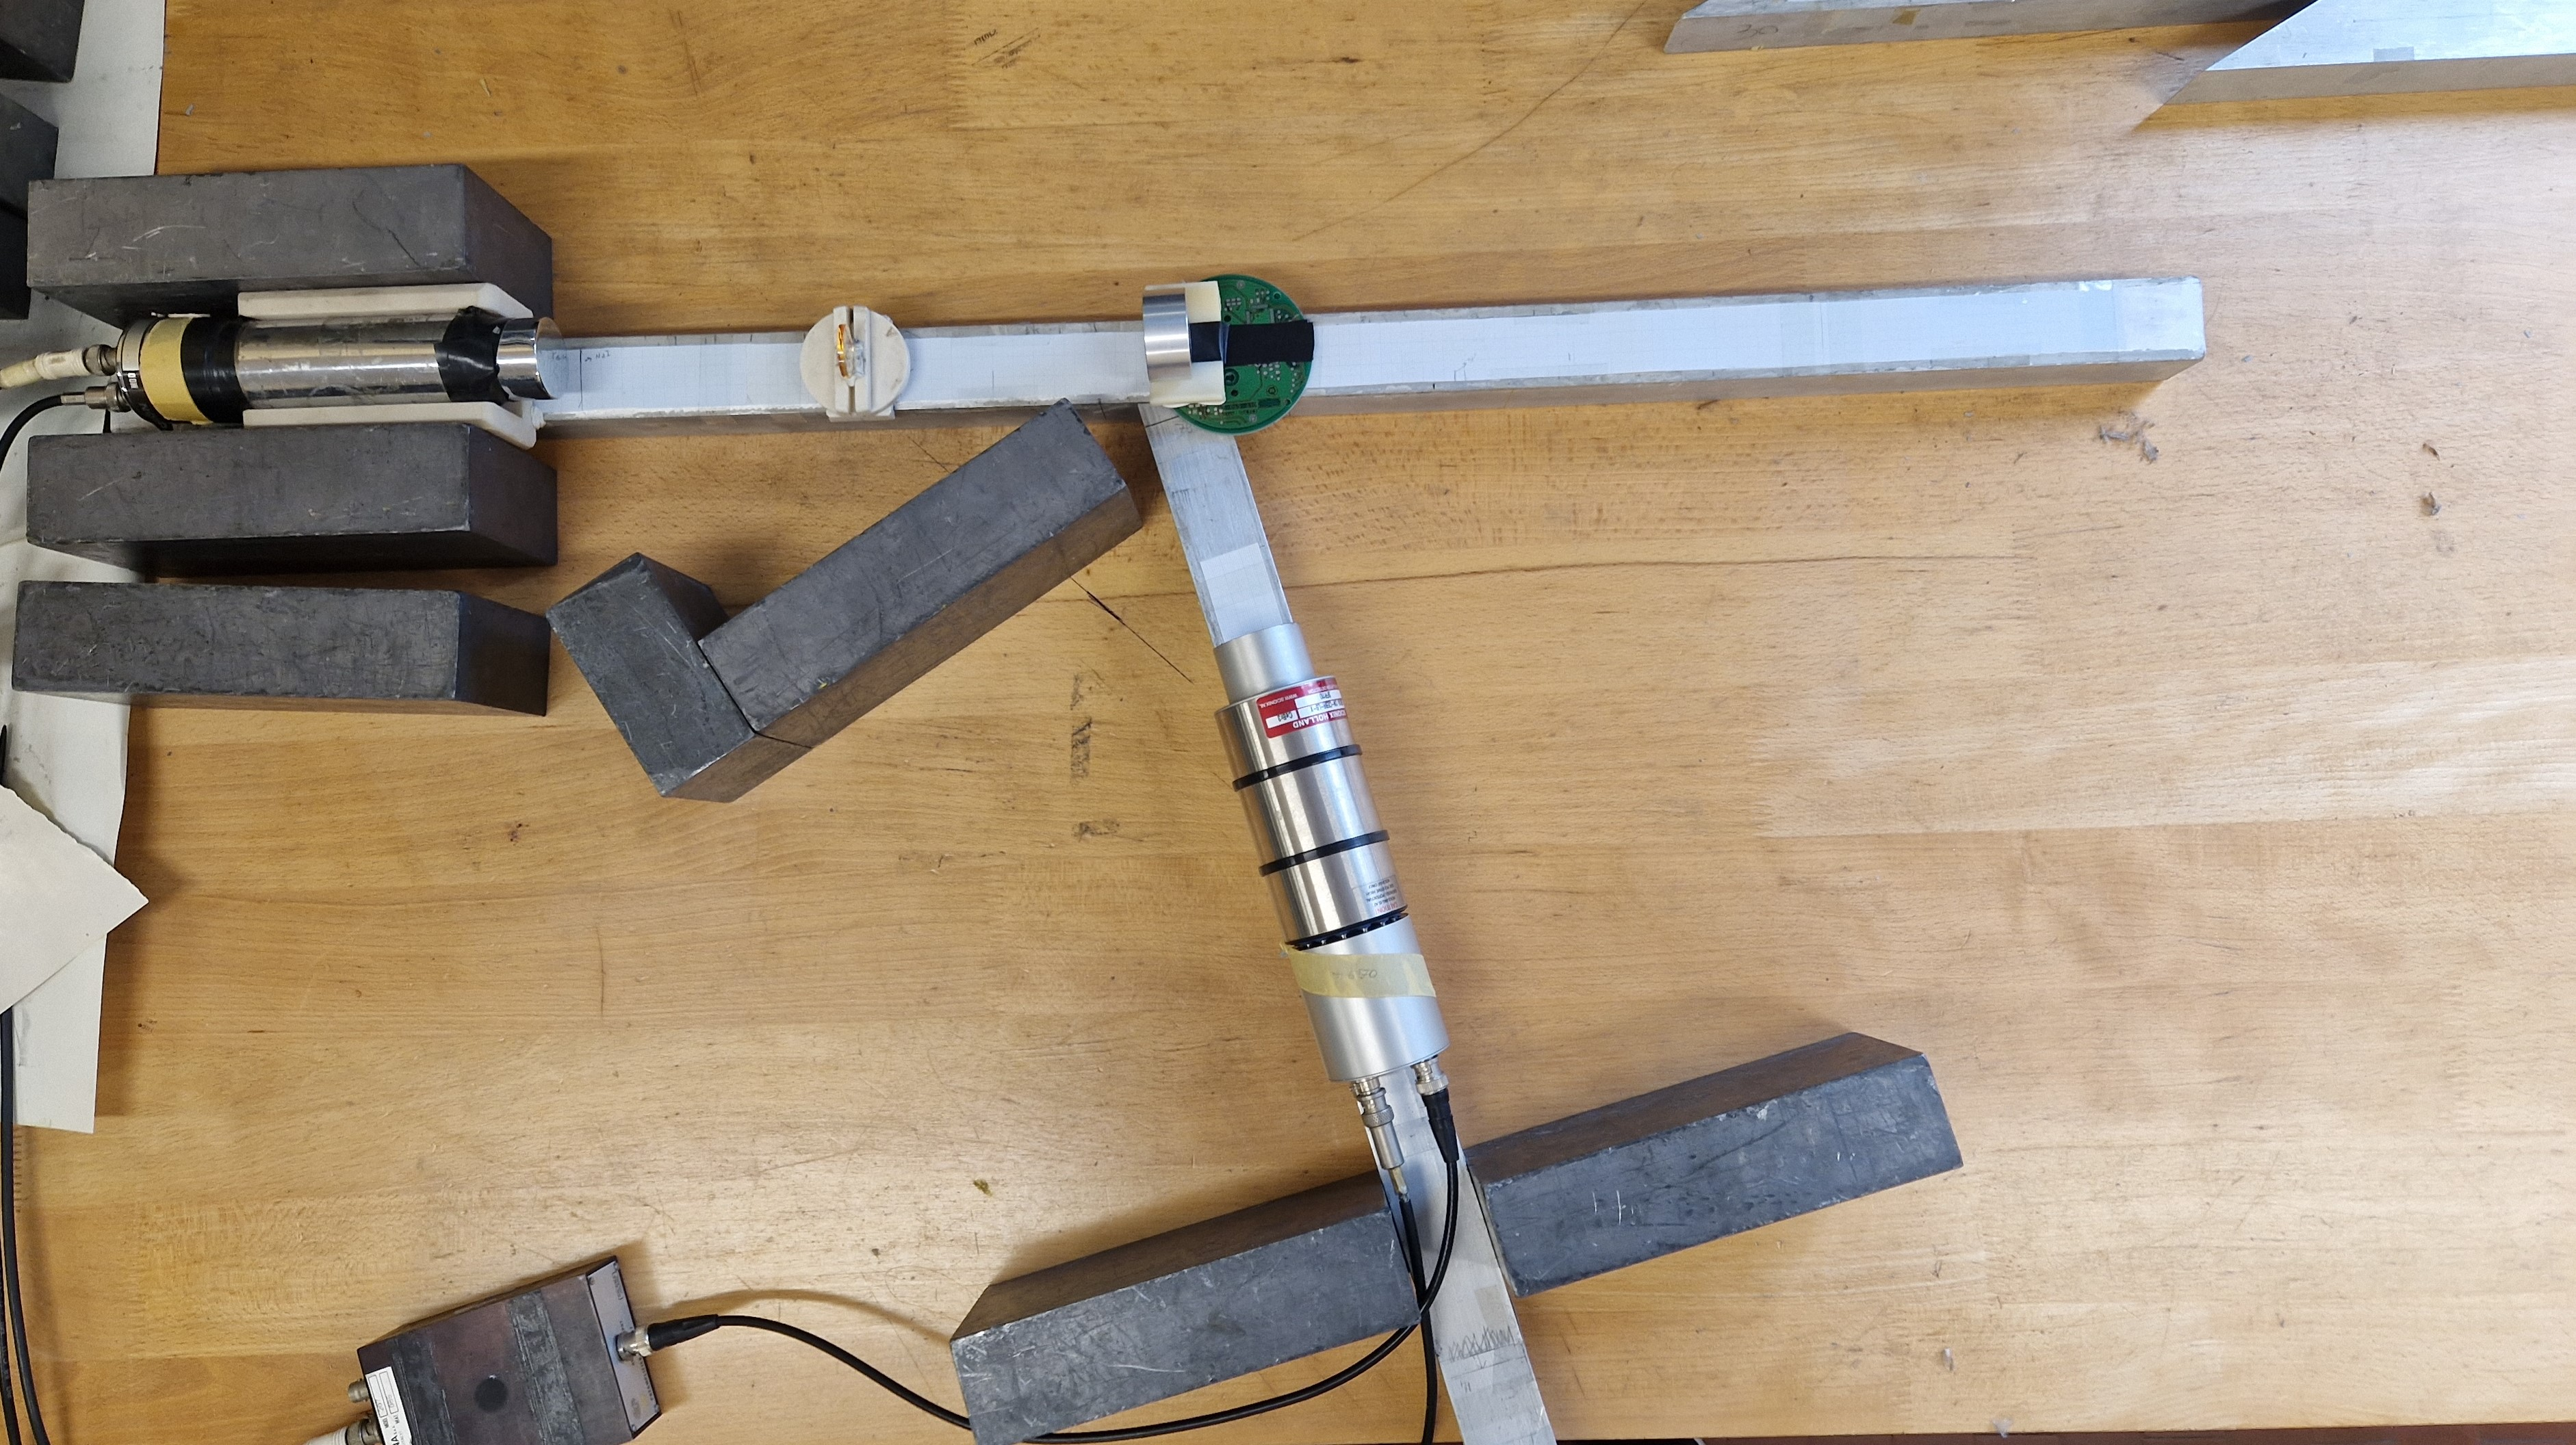
\includegraphics[scale=0.09]{Strumenti/apparato_sperimentale.jpg} 
  \caption{In questa immagine è possibile visualizzzare lo schema e la disposizione dell'apparato sperimentale durante una presa dati. Un'importante attenzione nei blocchi di $\ch{Pb}$ utilizzati sia per fissare i supporti ma anche per schermare i fotoni provenienti direttamente dalla sorgente.}
  \label{fig:apparato_sperimentale}
  %magari aggiungere delle didascalie all'interno dell'immagine o sostituire la foto con un disegno schematico
\end{figure}
Per assicurare un posizionamento stabile e preciso dei rivelatori, sono stati utilizzati dei supporti in metallo intagliati. Questi supporti hanno anche lo scopo di variare l'angolo di misura. Per quanto riguarda la sorgente e lo scatteratore, sono stati impiegati ulteriori supporti che hanno permesso un allineamento quantitativo di tutto il setup sperimentale. Tale allineamento è cruciale per minimizzare gli errori sistematici e ottenere dati affidabili. Le distanze sono scelte in modo che l'angolo solido sotteso allo scintillatore sia uguale rispetto all'angolo solido opposto che si forma con lo scatteratore. Oltre a questo è stata scelta una distanza molto maggiore rispetto ai raggi dei rivelatori in modo tale da porre l'apparato in buona geometria in modo da rendere trascurabile la frazione di radiazione secondaria che lo possa raggiungere. Ulteriori riflessioni sullo schema geometrico sono state affrontate in sezione \ref{sez_err_angolo_solido}
\subsection{Scelta del bersaglio}
Durante la fase preliminare dell'esperienza ci è stata data completa libertà sulla scelta del bersaglio. La selezione del materiale del bersaglio è stata effettuata considerando l'equazione che descrive il numero di fotoni scatterati:
\begin{equation}
     N_s = N_i \rho \frac{N_A}{M} Z dx \sigma(E)
     \label{eq:N_s}
\end{equation}
dove $\sigma$ è la sezione d'urto valutata per fotoni a $511\,\unit{keV}$, $N_s$ è il numero di fotoni scatterati, $N_i$ è il numero di fotoni incidenti, $\rho$ è la densità, $N_A$ la costante di Avogadro, $M$ è la massa molare del materiale, $Z$ è il numero atomico e $dx$ è lo spessore del bersaglio. I tre materiali presi in considerazione sono: alluminio, carbonio e rame.

A partire dai dati ottenuti attraverso il sito NIST XCOM\footnote{National Istitute of Standards and Technology: \url{https://physics.nist.gov/PhysRefData/Xcom/html/xcom1.html}} sono state fatte le seguenti considerazioni: per prima cosa, il rame è stato escluso poiché il contributo dell'effetto fotoelettrico è di un ordine di grandezza superiore rispetto a quello dell'alluminio e del carbonio, come è possibile visualizzare della tabella \ref{tab:bersagli}. Questo comporta che una significativa parte dei fotoni incidenti verrebbe assorbita piuttosto che scatterata, riducendo l'efficacia del bersaglio per lo scopo dell'esperimento.

\begin{table}[H]
    \centering
    \begin{tabular}{|c c c c|}
    \hline
    Elemento & $\sigma_{C}$ [\unit{\cm^{2}}] & $\sigma_{PH}$ [\unit{\cm^2}] & $\frac{\sigma_{C}}{\sigma_{TOT}}$ \\ [0.5ex] 
 \hline\hline
 Al & \num{2.860e-25} & \num{4.37e-28} & 99.19\% \\ 
 \hline
 C & \num{2.865e-25} & \num{2.15e-29} & 99.81\% \\ 
 \hline
 Cu & \num{2.848e-25} & \num{8.83e-27} & 94.67\% \\
 \hline 
    \end{tabular}
    \caption{Sezioni d'urto Compton (C) e Fotoelettrica (PH).}
    \label{tab:bersagli}
\end{table}
Successivamente è stato confrontato il carbonio e l'alluminio. Utilizzando l'equazione \ref{eq:N_s} è stato fatto un confronto tra il rapporto dei fotoni scatterati e incidenti con l'alluminio e il carbonio ottenendo i risultati visibili nella tebella (\ref{tab:considerazioni_finali}). Queste considerazioni ci hanno portato alla scelta finale dell'alluminio come bersaglio ottimale.
\begin{table}[H]
    \centering
    \begin{tabular}{|c c c c|}
    \hline
     Elemento & $\frac{N_s}{N_i}$ & $n_t dx \sigma$ & $\lambda_{COMP} [\unit{\cm}]$ \\ [0.5ex] 
 \hline\hline
 Al & 42.89\% & 0.4323 & 4.463 \\ 
 \hline
 C & 39.18\% & 0.392 & 5.117 \\ 
 \hline 
    \end{tabular}
    \caption{Confronto tra i fotoni scatterati utilizzando l'alluminio e il carbonio a parità di spessore ed energia dei fotoni.}
    \label{tab:considerazioni_finali}
\end{table}
Per quanto riguarda le dimensioni del bersaglio si è deciso di adottare come scatteratore un cilindro di alluminio di spessore pari a $2\, \unit{cm}$, che è circa la metà del valore di libero cammino medio dell'effetto Compton. La scelta di questa dimensione è dettata da due considerazioni principali: 
\begin{itemize}
    \item Massimizzare il rapporto $\frac{N_s}{N_i}$: un bersaglio con uno spessore sufficiente per ottenere un buon numero di fotoni scatterati, mantenendo un alto rapporto tra fotoni scatterati e incidenti.
    \item Assicurare un bersaglio sottile: mantenere $n_t \sigma dz << 1$ per evitare interazioni multiple e ridurre gli effetti di assorbimento all'interno del materiale. Un bersaglio sottile minimizza le probabilità di interazioni multiple dei fotoni con gli elettroni del bersaglio, garantendo che la maggior parte dei fotoni scatterati provengano da un singolo evento di scattering Compton.
\end{itemize}
Il bersaglio è stato intagliato da un cilindro di alluminio $6082$ utilizzando un tornio all'interno dell'officina nel dipartimento di fisca. L'alluminio serie $6000$ è anche conosciuto come anticorodal. 
\subsection{Geometria dell'apparato}
 Dal punto di vista sperimentale, le sezioni d'urto sono determinate per un angolo solido finito $\Delta \Omega$, che corrisponde all'angolo solido occupato dalla base del rivelatore cilindrico. L'angolo solido con cui un rivelatore di raggio $a$ "vede" una sorgente puntiforme posta a una distanza $d$ è dato da:
\begin{equation}
    \Omega=2\pi\left(1-\frac{d}{\sqrt{d^2+a^2}}\right)
\end{equation}
per $d>>a$ si approssima con:
\begin{equation}
    \Omega=\pi\frac{a^2}{d^2}
    \label{eq:angolo_solido}
\end{equation}
Le distanze tra i due rivelatori con la sorgente sono state quindi scelte in modo tale da eguagliare l'angolo solido sotteso. Questa configurazione assicura che ciascun rivelatore copra un volume angolare equivalente, migliorando la simmetria e la coerenza delle misure. Sono state fatte ulteriori considerazioni cercando di massimizzare l'efficienza di rivelazione studiata nella sezione dedicata \ref{eff}.

\section{Caratterizzazione della strumentazione}%titolo provvisorio
Per ottenere misurazioni ottimali, è stato necessario un lavoro preliminare per l'ottimizzazione della catena elettronica. I parametri regolabili includono: la tensione operativa dei due fotomoltiplicatori, il tempo di shaping per la modellazione dei segnali, la soglia $E_{\text{low}}$ e l'apertura $\Delta E$ della finestra del modulo ORTEC AMP\&SCA.
\subsection{Tensione di lavoro e shaping time}%l'italiano è orribile ma prima scrivo tutto poi cercherò di migliorare la forma, scusate ;(
Dopo aver svolto tutti i collegamenti tra i vari stadi elettronici esposti nella sezione (\ref{Elettronica nucleare}) si è collegato l'oscilloscopio all'uscita amplificata e formata del rivelatore A in modo da visualizzare il segnale uscente dopo l'amplificazione e la formazione. Dall'oscilloscopio è stato possibile eseguire un'ottimizzazione qualitativa direttamente sul segnale aumentando o diminuendo la tensione fornita al fotomoltiplicatore accoppiato con lo scintillatore e variando lo shaping time. In questo modo è stato possibile ricercare un segnale ottimale creando una situazione di compromesso tra la stabilità e la largezza. Il metodo è stato il seguente: stando attenti a non saturare il segnale si è aumentata la differenza di potenziale fornita dal generatore per aumentare l'ampiezza del segnale. Successivamente attraverso due manopole presenti nel modulo ORTEC RESEARCH AMPLIFIER è stato possibile modificare la  pendenza di risalita e discesa in modo tale da stringere il segnale. La tensione impostata per il primo rivelatore è stata scelta a $V_A=329\,\unit{V}$.

Svolgendo lo stesso procedimento per il secondo rivelatore è stata scelta come tensione $V_B=500\,\unit{V}$. Durante quest'ultimo processo si sono riscontrati alcuni problemi in quanto il rumore ambientale rendeva il segnale instabile e inutilizzabile. Per risolvere questo problema è stata aumentata la tensione fornita al fotomoltiplicatore in quanto questa agisce direttamente sul segnale prodotto dallo scintillatore. Tuttavia, a tensioni superiori a quella impostata, il segnale tendeva a saturare, motivo per cui è stata prestata particolare attenzione a evitare questa condizione.
\subsection{Calibrazione}\label{Sez calibrazione}
Il prossimo passo per ottimizzare la catena elettronica è quello di calibrare in energia entrambi i rivelatori. Infatti, il segnale di tensione analogico viene converito, tramite un Analog to Digital Converter (ADC), in un segnale digitale. Successivamente attraverso il Multy-Channel-Analyzer (MCA) i segnali vengono inseriti in un istogramma. Per questo motivo è necessario correlare la posizione nell'istogramma con il valore di energia rilasciata nel rivelatore, ovvero effettuare una calibrazione energetica. 

Questo può essere fatto utilizzando una sorgente avente picchi caratteristici dal valore noto e registrando la loro posizione nello spettro in canali. Le sorgenti utilizzate sono:
\begin{itemize}
    \item $\ch{^{22}Na}$ $(511\,\unit{keV})$;
    \item $\ch{^{137}Cs}$ $(661\,\unit{keV})$;
    \item $\ch{^{22}Ne}$ $(1274\,\unit{keV})$.
\end{itemize}
L'analisi dei picchi è affrontata nella sezione analisi dati (\ref{sez analisi dati calibrazione})
\subsection{Regolazione della finestra di energia}
Un altro passaggio fondamentale prima di iniziare con le misure è impostare la finestra di energia sul rivelatore B. Questo procedimento è fondamentale in quanto durante le misure i due rivelatori sono messi in coincidenza e per studiare l'effetto Compton si utilizzano i fotoni back-to-back prodotti dall'annichilazione del positrone con un elettrone. Di conseguenza attraverso il modulo SCA si può regolare la finestra di apertura in modo che sia centrata attorno al picco da $511\,\unit{keV}$. Questo permette al secondo rivelatore di essere utilizzato come ingresso di gate nel MCA. 

Sperimentalmente, con la sorgente posizionata al centro dell'apparato, è stato collegato il rivelatore B in modo tale da visualizzare lo spettro prodotto all'interno del software MAESTRO. Attraverso due manopole è stato possibile modificare la soglia e l'apertura della finestra. Visualizzando in tempo reale il formarsi dello spettro sullo schermo è stato possibile aggiustare i due parametri in modo tale da visualizzare solo il picco fotoelettrico. Durante questo pocedimento si è stata dedicata particolare attenzione a due fattori principali: la finestra non può essere troppo larga altrimenti si inquina lo spettro acquisito con coincidenze casuali, dall'altra parte non la si può stringere troppo per non abbattere eccessivamente il rate. Dopo aver impostato la finestra è stato necessario verificare che il segnale del fotone rilevato all'interno dello scintillatore A e il segnale logico di gate fossero nello stesso intervallo di tempo. Per fare questo è stato collegato al primo canale dell'oscilloscopio il segnale amplificato e formato del rivelatore A e nel secondo canale il segnale logico di gate come è possibile osservare nella fig. \ref{fig:osc}.
 %IMMAGINE osc
\begin{figure}[htp!]
  \centering
  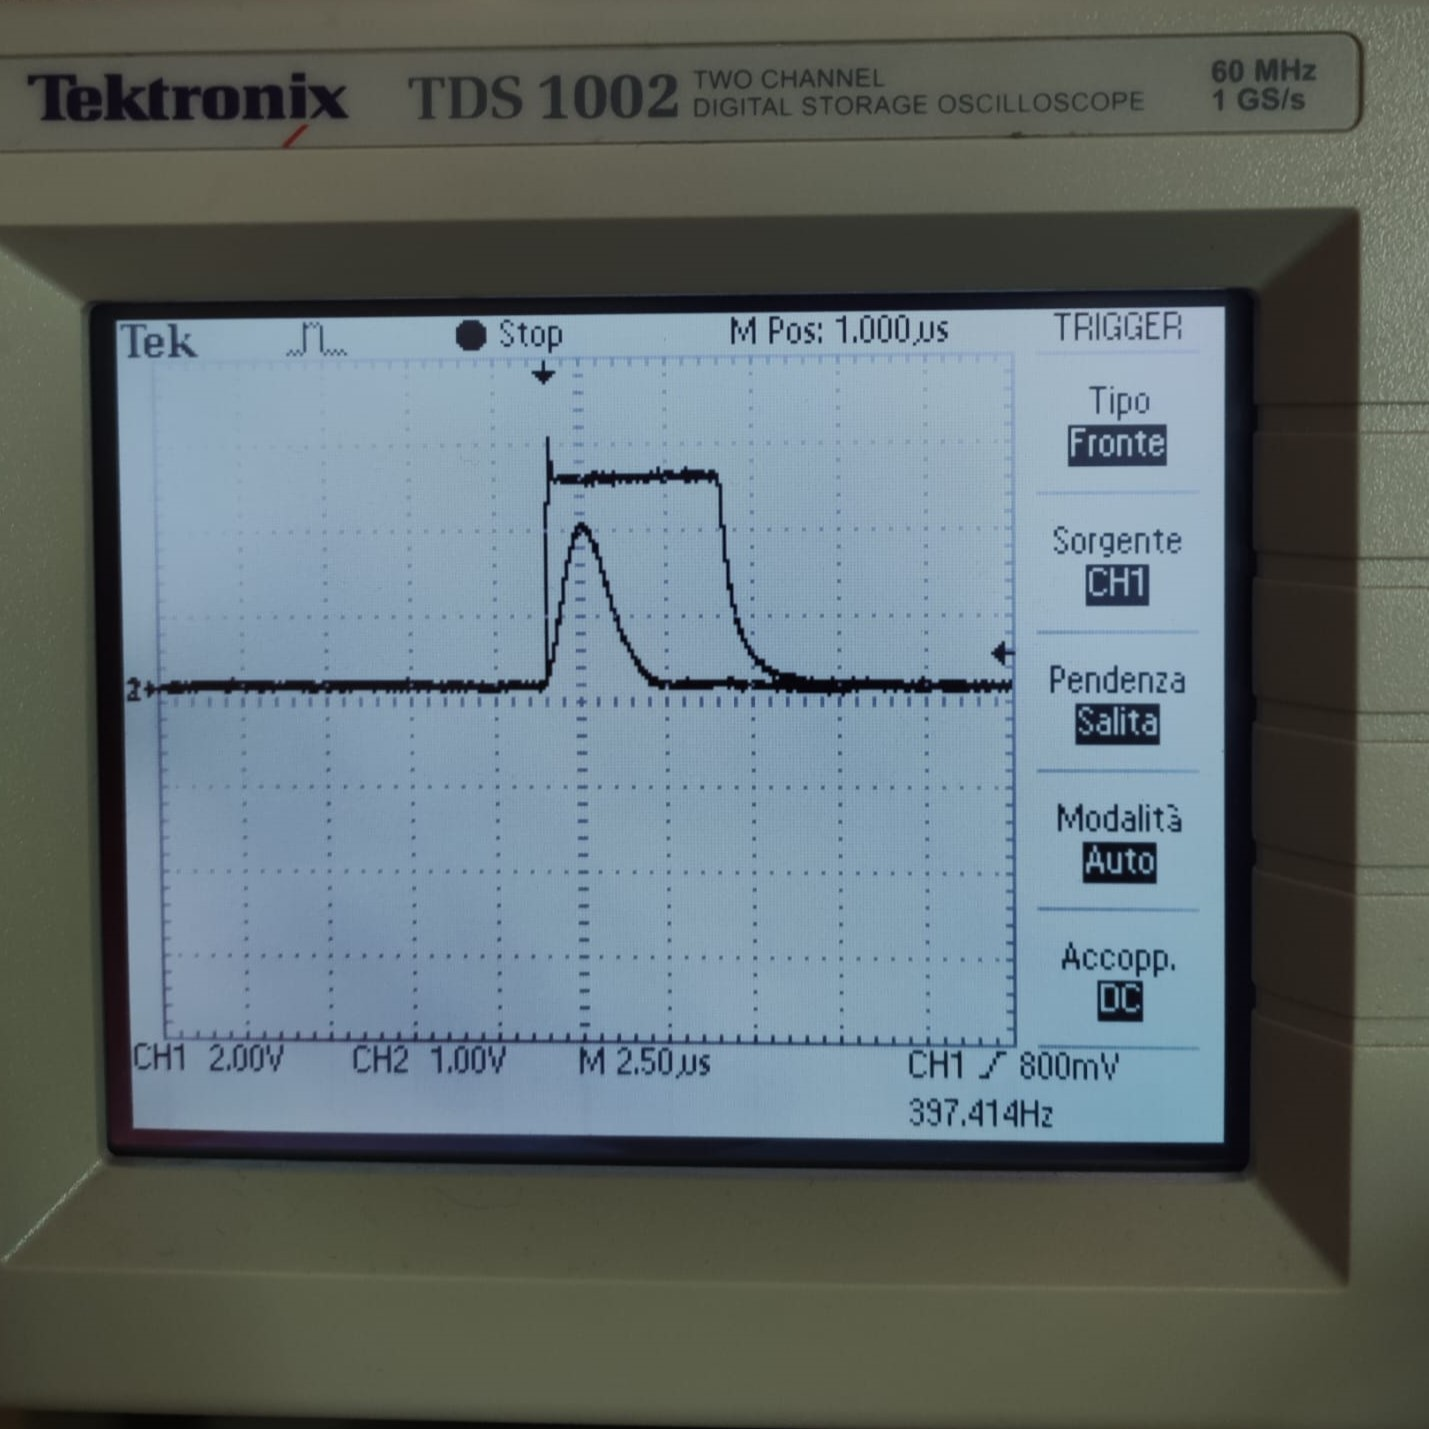
\includegraphics[scale=0.2]{Caratterizzazione della strumentazione/osc.jpg} 
  \caption{In questa immagine è possibile visualizzare la sovrapposizione del segnale del rivelatore A e del segnale logico di gate.}
  \label{fig:osc}
\end{figure}
\newpage
\section{Presa Dati}
\subsection{Efficienza dei rivelatori e distanze apparato sperimentale}\label{eff}
Per trovare l'efficienza totale dei rivelatori si è utilizzato lo schema in Figura \ref{immagine efficienza rivelatori}.
\begin{figure}[h]
    \centering
    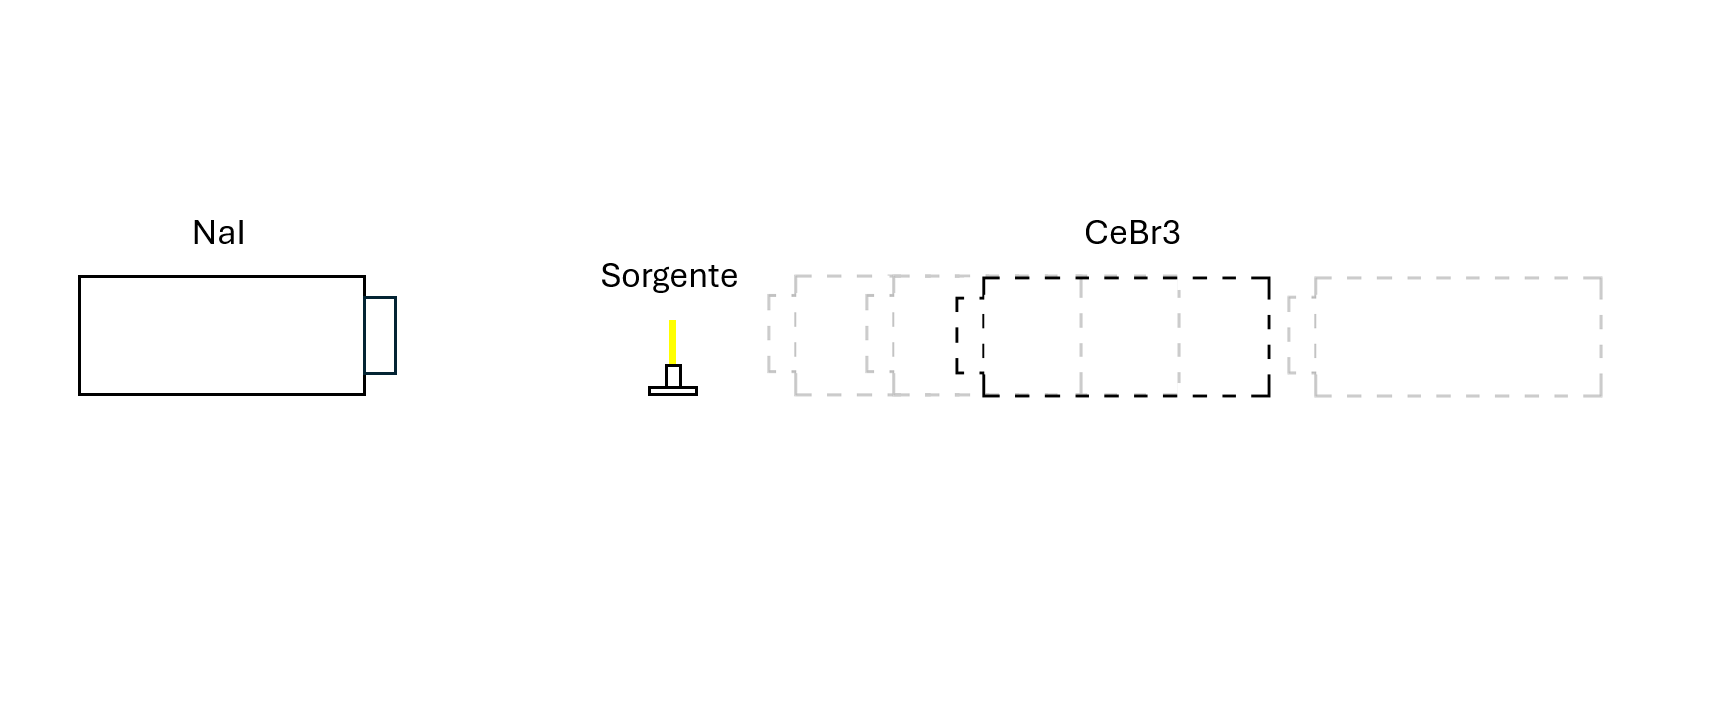
\includegraphics[width=0.85\textwidth]{Presa dati/Plateau efficienza.png}
    \caption{Raffigurazione della disposizione dei rivelatori per calcolare l'efficienza}
    \label{immagine efficienza rivelatori}
\end{figure}

Per calcolare l'efficienza totale dei rivelatori si è calcolato il rapporto tra i conteggi del rivelatore al $\ch{CeBr_{3}}$ ottenuti con l'aiuto del programma MAESTRO e i conteggi del gate, ovvero quelli rivelatore al $\ch{NaI}$ ottenuti mediante un contatore NIM; in formula:
\begin{equation}
    \text{Efficienza}_\text{tot}=\frac{\text{Conteggi}_{\ch{CeBr_3}}}{\text{Conteggi}_{\ch{NaI}}}
\end{equation}
Come si può notare dalla figura soprastante i conteggi sono stati ottenuti mantenendo fissa a $15 \,\unit{cm}$ la distanza tra la sorgente di $\ch{^{22}Na}$ e il rivelatore gate e spostando manualmente il rivelatore al $\ch{CeBr_3}$ a distanze fissate.
I valori sono stati presi in un intervallo di tempo di 60 secondi per ogni misura e sono riportati in tabella \ref{tabella efficienza}.
\begin{table}[H]
    \centering
    \begin{tabular}{|c|c|c|c|}
    \hline
       dist. $\ch{CeBr_{3}}$-sorgente [$\unit{cm}$] & cont. $\ch{CeBr_{3}}$ & cont. gate ($\ch{NAI}$) & Efficienza (\%) \\
    \hline
    \hline
    $7$ & $11095$ & $17746$ & $62.52$ \\
    \hline
    $14$ & $11007$ & $18062$ & $60.94$ \\
    \hline
    $15$ & $10897$ & $17770$ & $61.32$ \\
    \hline
    $16$ & $10817$ & $18154$ & $59.58$ \\
    \hline
    $17$ & $10582$ & $18120$ & $58.40$ \\
    \hline
    $18$ & $9553$ & $17834$ & $59.34$ \\
    \hline
    $20$ & $9231$ & $18041$ & $51.17$ \\
    \hline
    $30$ & $4667$ & $17982$ & $25.95$ \\
    \hline
    \end{tabular}
    \caption{Sono presentati i vari valori utilizati per il calcolo dell'efficienza dei rivelatori.}
    \label{tabella efficienza}
\end{table}
Nel grafico sottostante si può notare come si formi il cosiddetto \textit{plateau} intorno a $15 \,\unit{cm}$.
\begin{figure}[H]
  \centering
  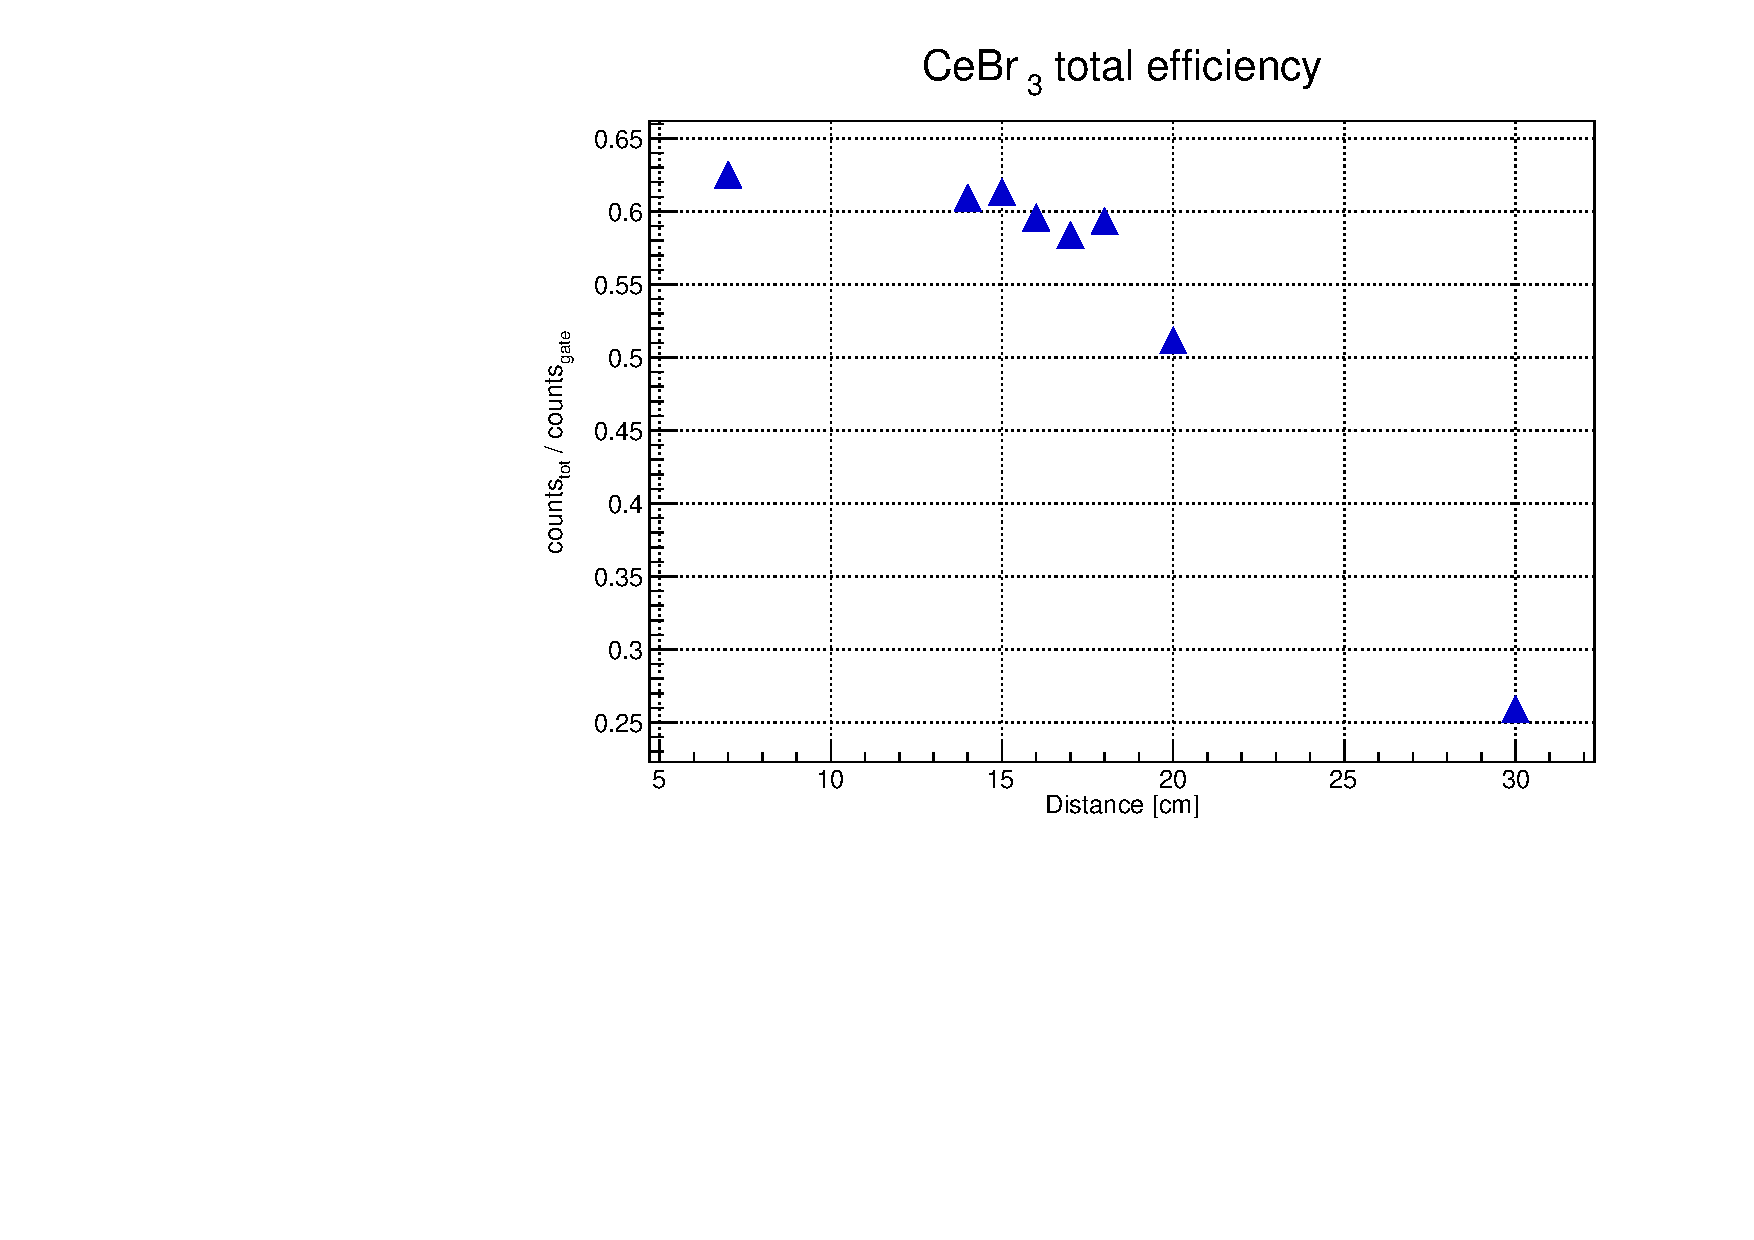
\includegraphics[scale=0.6]{Analisi Dati/tot_eff.pdf} 
  \caption{Plateau dell'efficienza del rivelatore}
  \label{fig:eff_tot}
\end{figure}
Date le considerazioni della sezione precedente si è deciso di fissare la distanza tra sorgente e $\ch{CeBr_{3}}$ a $15 \,\unit{cm}$ per vari motivi: prima di tutto perché è dove si trova il plateu; in secondo luogo perché mettendolo troppo vicino si osserverebbero effetti di \textit{pile-up} e il rivelatore vedrebbe anche particelle deviate a grande angolo pur non essendo angolato.
Inolre questo è un valore comodo per le altre lunghezze presenti nell'apparato sperimentale: infatti si sono calcolate le distanze tra sorgente e $\ch{NaI}$ e tra bersaglio e $\ch{CeBr_{3}}$ in modo tale da aver lo stesso angolo solido che si ha tra la sorgente e il bersaglio posto a $15\,\unit{cm}$. Per il calcolo degli angoli solidi tra la sorgente e bersaglio e tra sorgente e $\ch{NaI}$ la sorgente è stata considerata puntiforme, mentre per l'angolo solido tra bersaglio e rivelatore $\ch{CeBr_{3}}$ è stato considerato puntiforme e centrato il punto di interazione del fotone con il bersaglio di $\ch{Al}$. I valori delle distanze ottenuti sono riportati nella tabella sottostante.
\begin{table}[H]
    \centering
    \begin{tabular}{|c|c|}
    \hline
    $\text{Distanza} \quad \ch{NaI}-\text{sorgente}$ & $13.5\, \unit{cm}$ \\
    \hline
    $\text{Distanza} \quad \text{sorgente}-\text{bersaglio} (\text{fissata})$ & $15 \,\unit{cm}$ \\
    \hline
    $\text{Distanza} \quad \text{bersaglio}-\ch{CeBr_{3}}$ & $14.4\,\unit{cm}$ \\
    \hline
    \end{tabular}
    \caption{Sono presentati i vari valori delle distanze dell'apparato sperimentale.}
    \label{tabella efficienza}
\end{table}
%sarebbe utile indicare nella tabella come abbiamo chiamato le varie distanze. Quindi con l o d 
Per l'efficienza fotoelettrica sono state utilizzate le stesse misure dell'efficienza totale con la differenza che attraverso l'analisi dati si sono selezionati solo i conteggi del picco fotoelettrico. I valori ottenuti sono riportati nel grafico sottostante.
\begin{figure}[H]
  \centering
  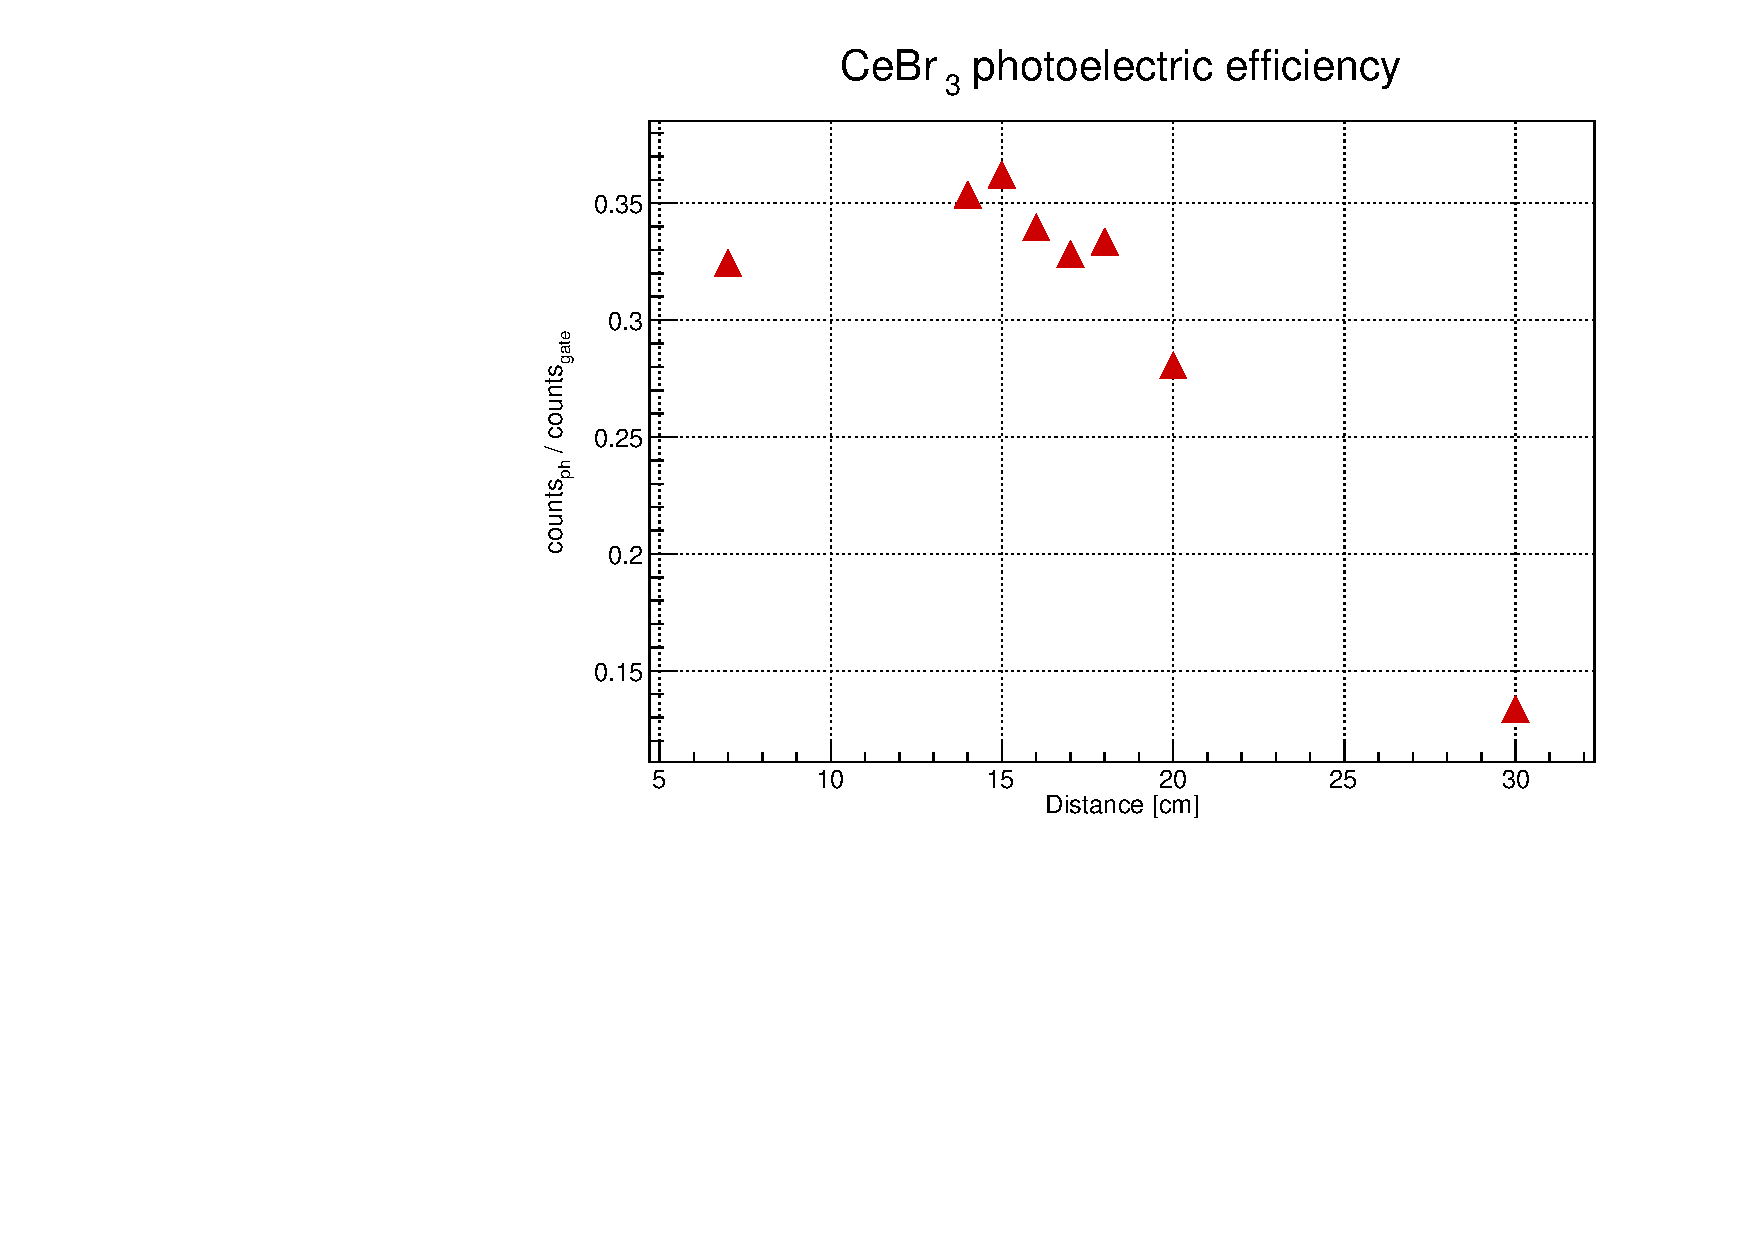
\includegraphics[scale=0.6]{Analisi Dati/ph_eff.pdf} 
  \caption{Plateau dell'efficienza fotoelettrica del rivelatore}
  \label{fig:eff_ph}
\end{figure}
\subsection{Misure della sezione d'urto}
Per quel che riguarda le misure a vari angoli sono stati stabiliti i valori di $30^\circ$, $45^\circ$, $60^\circ$ e $90^\circ$. Per uniformità tra le varie misure si è deciso di segnare sulla carta millimetrata il centro del bersaglio; questo è stato punto di riferimento dal quale sono state prese le misure di distanza bersaglio-rivelatore A nelle misure a vari angoli. Come visibile in fig. \ref{fig:schema_misura_distanze} il punto marcato ha consentito di misurare la distanza $l$ %non si capisce bene che cosa rappresenta la distanza l
a partire dal centro del bersaglio; inoltre risultava comodo per misurare accuratamente la disposizione angolare tramite il goniometro.

\begin{figure}[H]
    \centering
    \includegraphics[scale=0.15]{Errori/schema_distanze.png}
    \caption{Schematizzazione delle misure delle distanze. In rosso: distanza sorgente - bersaglio. In verde: distanza bersaglio - rivelatore A.}
    \label{fig:schema_misura_distanze}
\end{figure}
Le prese dati sono durate svariate ore a seconda del valore dell'angolo che veniva misurato e i valori di sezione d'urto, calolati con la formula \ref{eq sezione d'urto conteggi}, sono riportati nella Tabella \ref{tabella sezione d'urto}.
Inizialmente erano stati presi i dati anche per misure di $75^\circ$ e $120^\circ$, ma dopo qualche giorno di presa dati ci siamo subito accorti che i conteggi rilevati dal modulo \textit{NIM} subivano un reset dopo un certo tempo trascorso, probabilmente legato alla capacitá di memoria disponibile nel modulo stesso. A causa di ció le uniche misure di conteggi utilizzabili sono risultate quelle a $30^\circ$, $45^\circ$, $60^\circ$ e $90^\circ$ in quanto erano state effettuate in un tempo tale da non subire il reset del counter.
\begin{table}[H]
    \centering
    \begin{tabular}{|c|c|c|}
    \hline
       Angolo & $d\sigma/d\theta$ [$\num{e-26}\unit{cm^{2}/sr}$] & Errore sezione d'urto [$\num{e-27}\unit{cm^{2}/sr}$] \\
    \hline
    \hline
    $30^\circ$ & $3.92$ & $5.58$ \\
    \hline
    $45^\circ$ & $3.15$ & $4.48$ \\
    \hline
    $60^\circ$ & $2.50$ & $3.56$ \\
    \hline
    $90^\circ$ & $1.92$ & $2.73$ \\
    \hline
    \end{tabular}
    \caption{Sono presentati i vari valori ottenuti per la sezione d'urto.}
    \label{tabella sezione d'urto}
\end{table}
Gli errori associati alle misure e l'analisi dati sono esposti nella sezione \ref{sezione d'urto e montecarlo}.
\newpage
\section{Analisi Dati}
\subsection{Analisi degli Spettri}\label{sez analisi dati calibrazione}
Per calibrare in energia il \textit{Multi-Channel-Analyzer} sono stati presi due spettri, uno con la sorgente sperimentale $\ch{^{22}Na}$ ed uno con una sorgente di $\ch{^{137}Cs}$ .
I dati istogrammati sono poi stati analizzati tramite \textit{ROOT}\footnote{Codice consultabile al seguente link: \url{https://gitfront.io/r/MicheleScattola/GaGvFGBPX4Vm/Misure-Nucleari/tree/Compton/}}. Attorno al picco di emissione viene eseguito un fit Gaussiano al quale è aggiunto un fondo lineare. Per ottimizzare la regione di spettro su cui effettuare il fit viene prima stimato all'interno del codice il picco e la \textit{FWHM} tramite i bin dell'istogramma. Si riesce dunque ad effettuare il fit gaussiano in un intervallo di $\pm 3 \sigma$ attorno al picco ed inizializzando i parametri di fit con le stime iniziali.

I dati estrapolati dagli spettri di $\mu$ e $\sigma$ sono stati utilizzati per effettuare la calibrazione lineare in energia dei canali MCA.
Per quanto riguarda gli errori sui valori teorici si è fatto riferimento al \textit{National Nuclear Data Center (NNDC)}\footnote{\url{https://www.nndc.bnl.gov/nudat3/}}; i dati completi sono riportati in appendice in tabella \ref{tab:ADC} . Si è dunque eseguito un fit (fig. \ref{fig:calibrazioneADC}) del tipo $y = ax + b$ ; i parametri sono poi stati utilizzati per convertire le successive misure da canali ADC ad energia.
\begin{figure}[H]
  \centering
  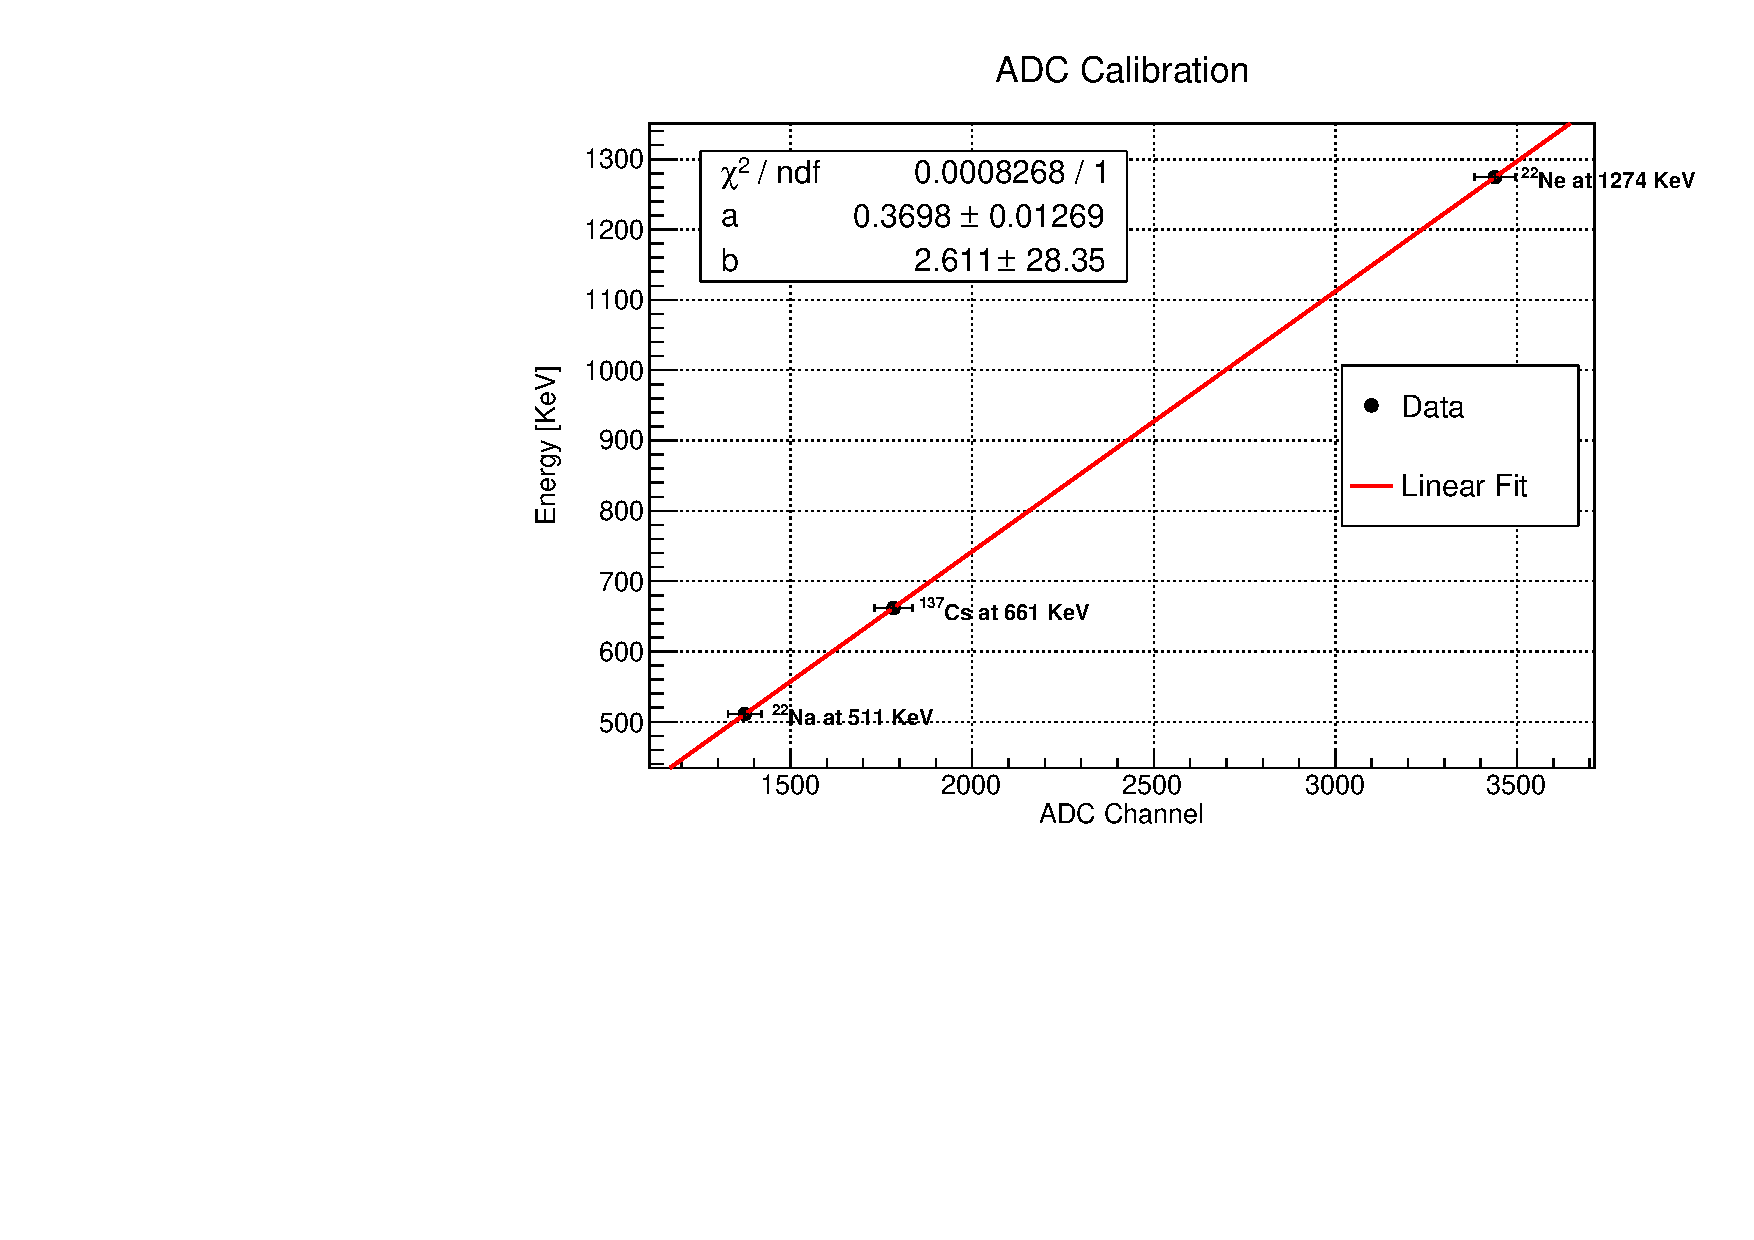
\includegraphics[scale=0.5]{Analisi Dati/linear.pdf} 
  \caption{Calibrazione ADC}
  \label{fig:calibrazioneADC}
\end{figure}
In seguito gli spettri acquisiti ai vari angoli $\theta$ sono stati analizzati in modo analogo al metodo utilizzato per la calibrazione, convertendo i canali ADC in Energia. L'analisi ha facilmente verificato lo spostamento del picco fotoelettrico; tutti gli spettri sono riportati in appendice \ref{appendice_spettri}, viene riportato in fig. \ref{fig:spettro60} quello ottenuto a 60 gradi.
\begin{figure}[H]
  \centering
  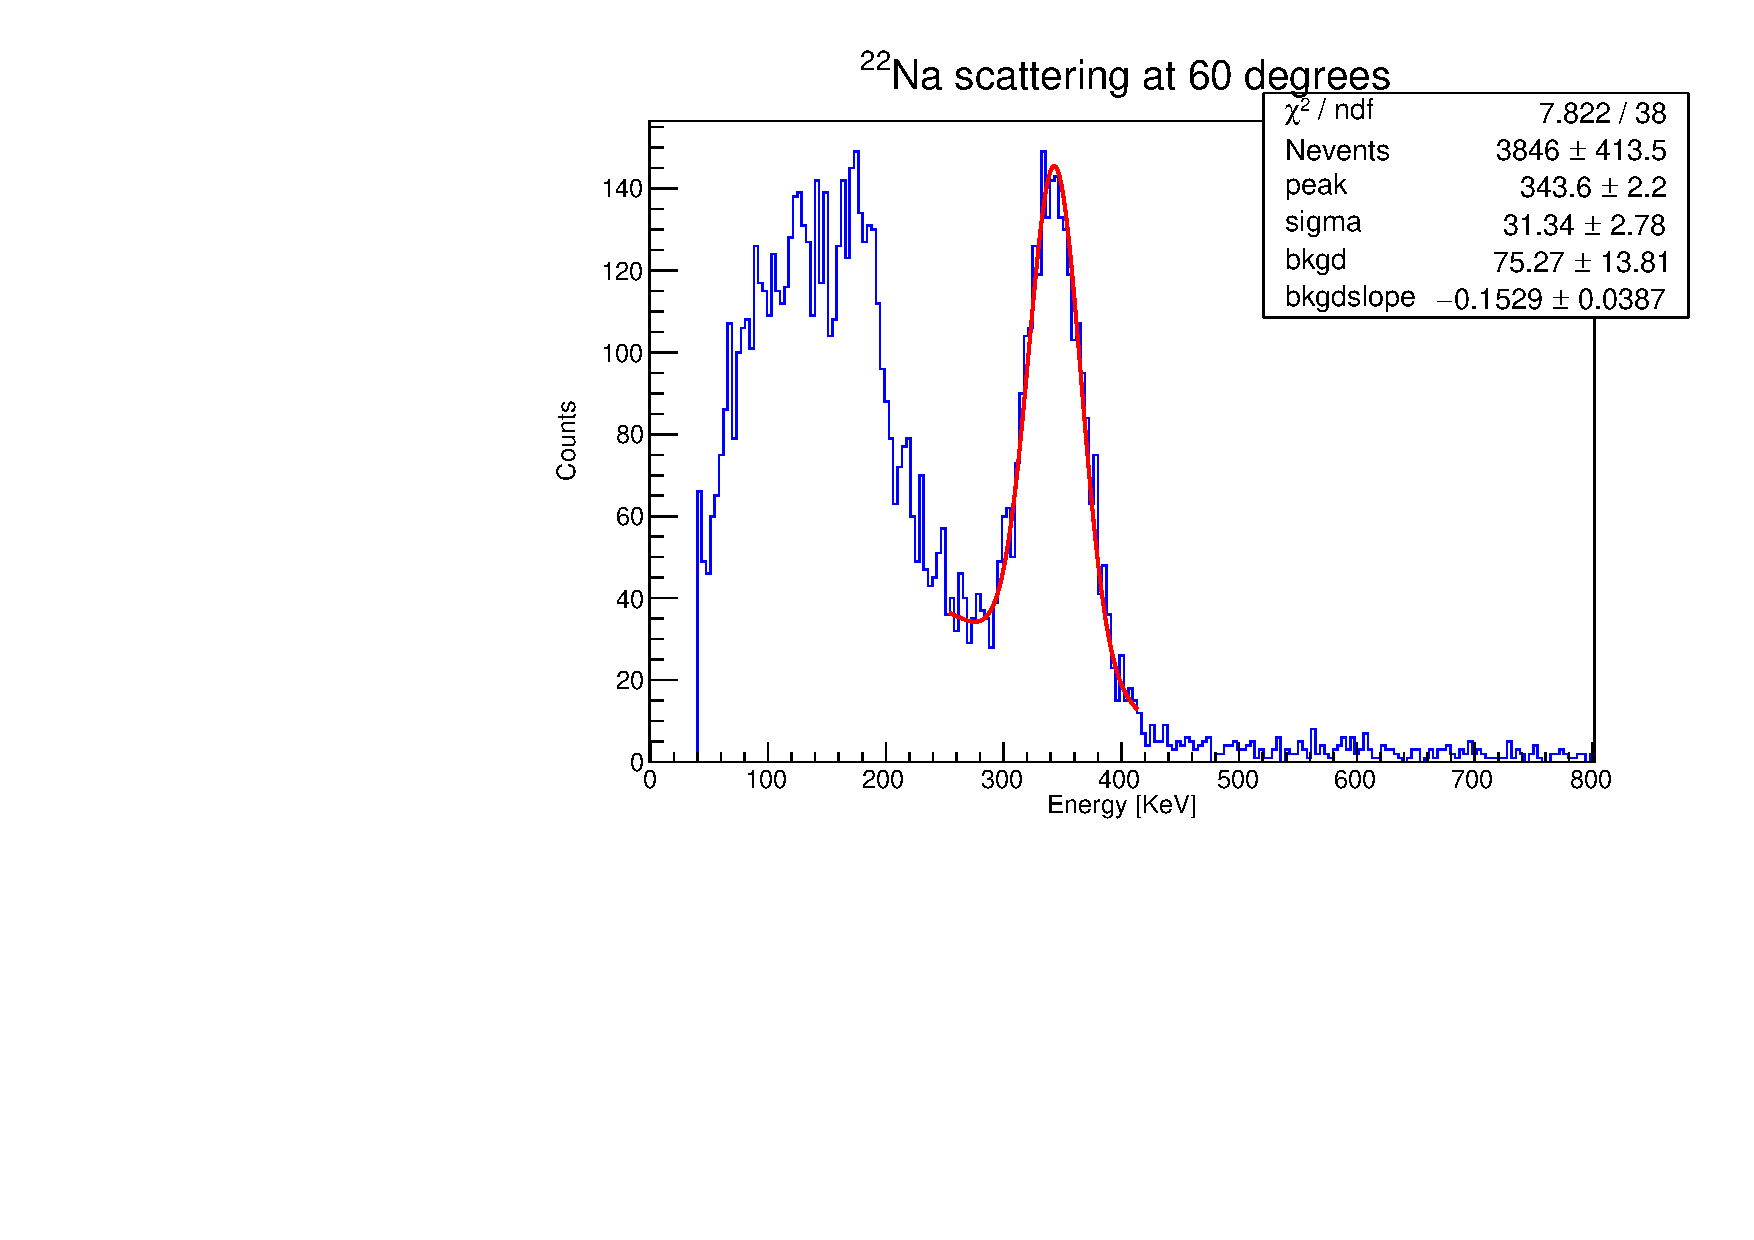
\includegraphics[scale=0.45]{Appendice/60_deg_spectrum.pdf} 
  \caption{Spettro acquisito a 60 gradi}
  \label{fig:spettro60}
\end{figure}
\subsection{Energia del fotone}
I dati estrapolati dagli spettri hanno permesso di rappresentare in fig. \ref{fig:E_gamma} l'energia del fotone uscente rispetto all'angolo di scattering - eq. \eqref{energia fotone uscente} . L'incertezza per i picchi è data da $\sigma_{TOT} = \frac{\sigma}{\sqrt{N}}$ dove N sono i conteggi sotto al picco e $\sigma$ la larghezza gaussiana. Queste incertezze risultano tuttavia considerevolmente minori rispetto a quelle relative alla posizione angolare e non sono dunque visibili nel grafico. I risultati completi sono disponibili in tabella in appendice \ref{tab:appendice_spettri}.
\begin{figure}[H]
  \centering
  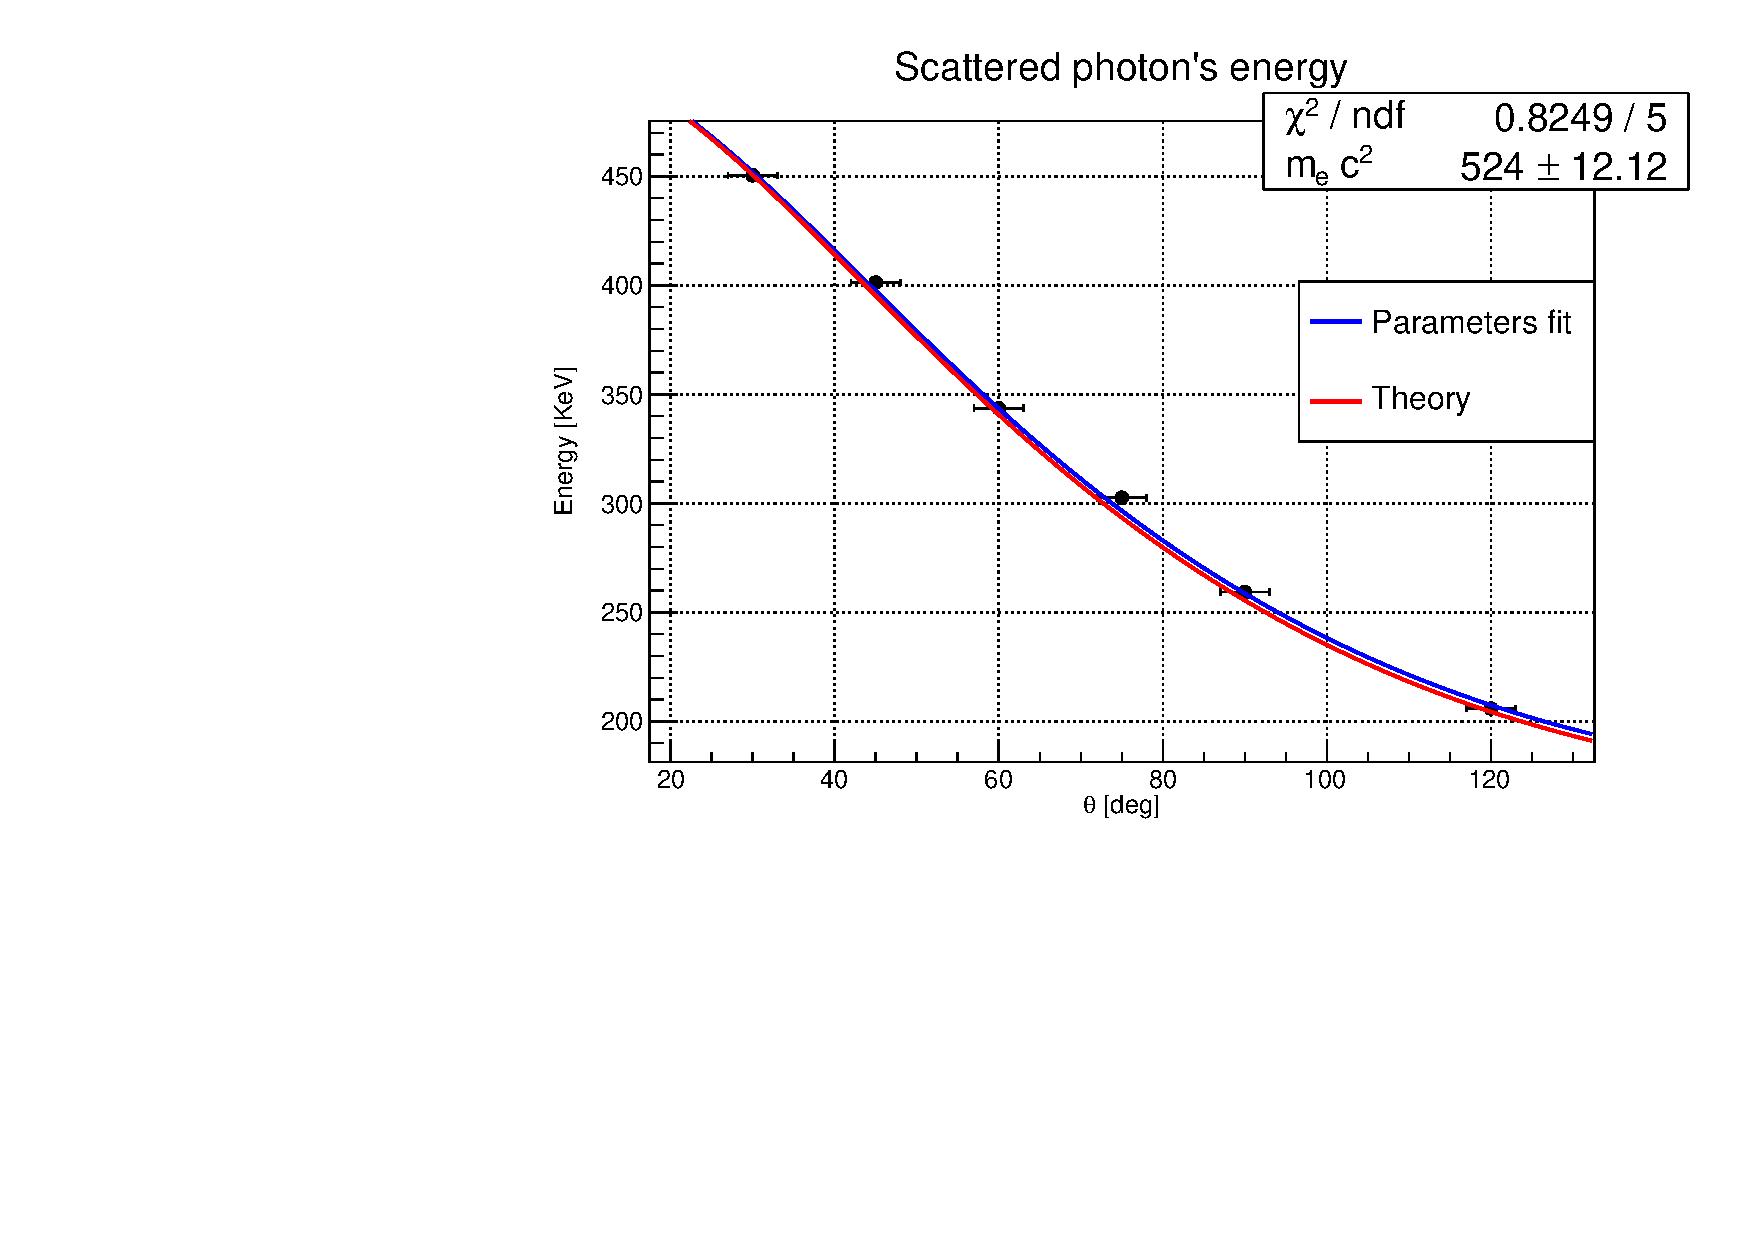
\includegraphics[scale=0.6]{Analisi Dati/E_1.pdf} 
  \caption{Ricostruzione della curva in energia del fotone uscente}
  \label{fig:E_gamma}
\end{figure}
Sono stati eseguiti due fit , i cui risultati sono riportati in tabella \ref{tab:risultati_energia}: il primo  relativo alla curva teorica ed il secondo lasciando come parametro libero il termine $m_e c^2$. Si nota inoltre che la curva parametrica si sovrappone a quella teorica confermando la bontà del risultato.
\begin{table}[H]
    \centering
    \begin{tabular}{|c c c c c|}
    \hline
    Tipo di fit & $\chi^2$ & $ndf$ & Probabilità  & $m_e c^2$ [\unit{\kilo\electronvolt}]\\ [0.5ex] 
 \hline\hline
 Teorico & 2.00 & 6 & 91.95 \% & 511 \\ 
 \hline
 Parametrico & 0.825 & 5 & 97.54 \% & $523\pm12$\\ 
 \hline 
    \end{tabular}
    \caption{Risultati di fit per l'energia del fotone uscente.}
    \label{tab:risultati_energia}
\end{table}
Si riferisce inoltre che lo spettro a 0 gradi è stato omesso dal grafico in seguito ad alcune considerazioni. Si notava infatti subito che fosse distaccato considerevolmente dal valore teorico ed avendo acquisito molti eventi vi è associata una incertezza molto piccola. Questo perchè la misura è stata effettuata alla fine dell'esperienza ad alcuni giorni di distanza da quelle precedenti e probabilmente le condizioni ambientali hanno modificato il comportamento sperimentale. Sarebbe stato dunque necessario effettuare una nuova calibrazione.
\subsection{Sezione d'urto}
Dalle misure sperimentali si è poi ricostruita la sezione d'urto data l'eq. \ref{eq sezione d'urto conteggi}. In seguito alle considerazioni in sezione \ref{sez_err_conteggi} le uniche misure utilizzabili per quanto riguarda i conteggi sono quelle a $30^\circ$, $45^\circ$, $60^\circ$ e $90^\circ$. L'errore associato alla misura è stato valutato tramite propagazione degli errori, la cui analisi viene affrontata in sezione \ref{sez_errori}. I dati ottenuti sono rappresentati in figura \ref{fig:sezione_sperimentale}.
\begin{figure}[H]
  \centering
  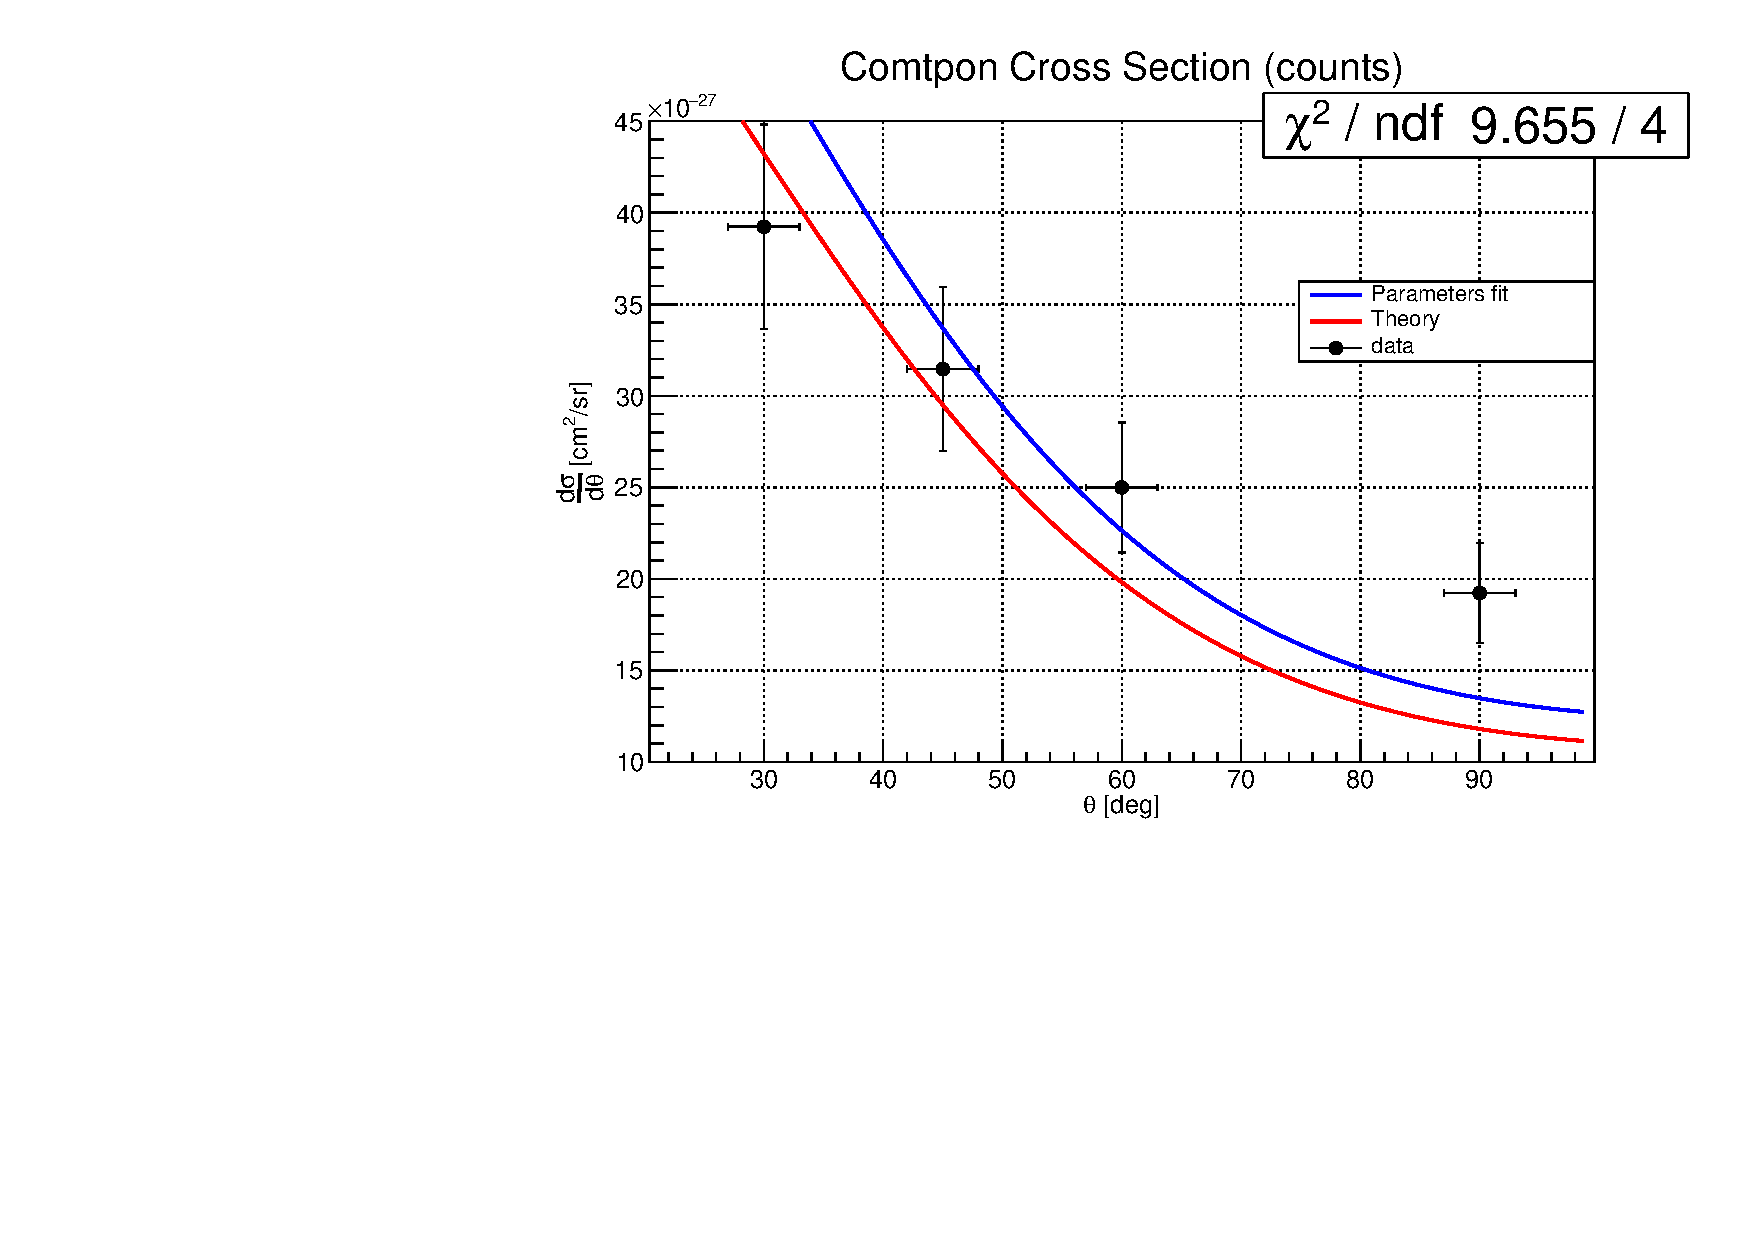
\includegraphics[scale=0.6]{Analisi Dati/ExpCrossSec_counts.pdf} 
  \caption{Ricostruzione della sezione d'urto Compton tramite i conteggi}
  \label{fig:sezione_sperimentale}
\end{figure}
Sui dati vengono eseguiti due fit analogamente a quanto fatto per l'energia del fotone uscente, i cui risultati sono disponibili in tabella \ref{tab:risultati_sezione}. In questo caso il parametro libero è il raggio classico dell'elettrone $r_e$.
\begin{table}[H]
    \centering
    \begin{tabular}{|c c c c c|}
    \hline
    Tipo di fit & $\chi^2$ & $ndf$ & Probabilità  & $r_e$ [fm]\\ [0.5ex] 
 \hline\hline
 Teorico & 9.65 & 4 & 4.76 \% & $\num{2.8179}$ \\ 
 \hline
 Parametrico & 7.31 & 3 & 6.27 \% & $\num{3.01}\pm\num{0.65}$\\ 
 \hline 
    \end{tabular}
    \caption{Risultati di fit per la sezione d'urto Compton.}
    \label{tab:risultati_sezione}
\end{table}

%Inoltre è stato possibile ricavare una stima della sezione d'urto tramite la formula di Klein-Nishina (\ref{eq sezione d'urto Klein-Nishina}) , utilizzando i picchi degli spettri acquisiti ai vari angoli. L'errore considerato proviene direttamente dalla propagazione degli errori visibile in appendice \ref{appendice_errore_sezione_energie}.
%\begin{figure}[H]
  %\centering
  %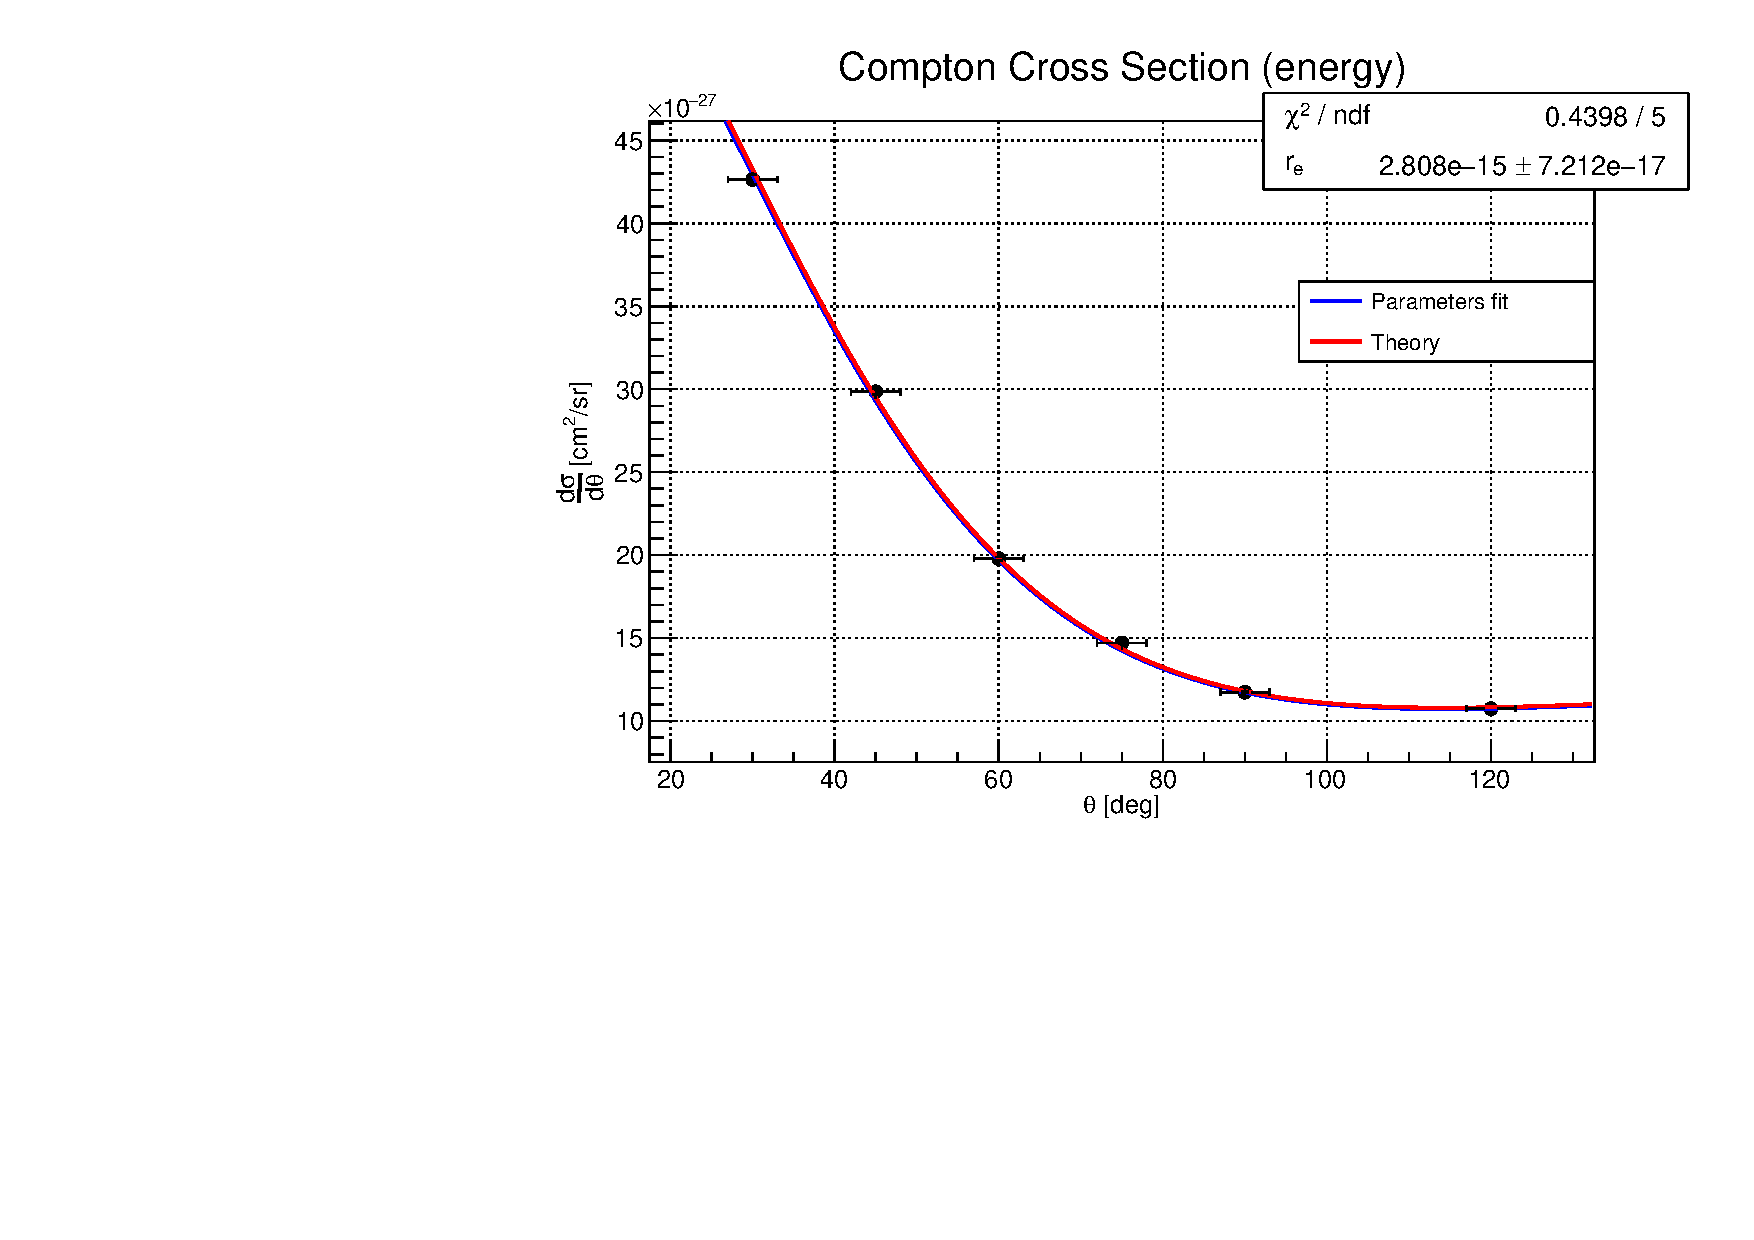
\includegraphics[scale=0.6]{Analisi Dati/ExpCrossSec_energy.pdf} 
  %\caption{Ricostruzione della sezione d'urto Compton tramite i picchi di energia}
  %\label{fig:sezione_energie}
%\end{figure}
%Analogamente a quanto fatto per i conteggi vi sono due fit che riproducono i seguenti risultati:
%\begin{table}[H]
   % \centering
   % \begin{tabular}{|c c c c c|}
   % \hline
   % Tipo di fit & $\chi^2$ & $ndf$ & Probabilità  & $r_e$ [fm]\\ [0.5ex] 
 %\hline\hline
 %Teorico & 7.99 & 6 & 24 \% & $\num{2.8179}$ \\ 
% \hline
% Parametrico & 0.439 & 5 & 99 \% & $\num{2.81}\pm\num{0.07}$\\ 
 %\hline 
 %   \end{tabular}
  %  \caption{Risultati di fit per la sezione d'urto Compton.}
    %\label{tab:risultati_sezione}
%\end{table}
%Si nota subito come le incertezze non siano visibili, in quanto nell'ordine di grandezza di $\num{e-28}\,\unit{\cm^{-2}}$ . Questo risulta dal fatto che le uniche incertezze coinvolte sono quelle relative ai picchi di energia e quella dell'angolo di scattering; quest'ultima in particolare risulta molto poco influente sul risultato.
%La stima del parametro $r_e$ risulta infine migliorata rispetto a quella precedente.


\newpage
\section{Trattazione degli errori}\label{sez_errori}
\subsection{Conteggi}\label{sez_err_conteggi}
Per la determinazione dell'errore sui conteggi, abbiamo utilizzato la radice quadrata dei conteggi stessi, in accordo con la statistica di Poisson. Pertanto, per l'errore associato al numero di conteggi, ovvero per $\sigma_{N_{s}}$, abbiamo preso $\sqrt{N_{S}}$ mentre per $\sigma_{N_{i}}$ abbiamo preso $\sqrt{N_{i}}$. Oltre a questo è importante prestare attenzione ad un errore sistematico presente in ogni misura legato alla scelta dell'intervallo di integrazione dello spettro.

Il termine $N_s/N_i$ che compare all'iterno della formula della sezio d'urto differenziale (\ref{eq sezione d'urto conteggi}) è composta da due misure correlate tra di loro di conseguenza trattandola come una binomiale si ottiene che l'errore su questo rapporto è:
\begin{equation}
    \sigma_{\frac{N_s}{N_i}}=\frac{1}{N_i}\sqrt{N_s\left(1-\frac{N_s}{N_i}\right)}
\end{equation}
\subsection{Angolo solido}\label{sez_err_angolo_solido}
Per quanto riguarda la misura dell'angolo solido l'errore è stato inizialmente calcolato tramite propagazione della relazione geometrica introdotta in eq. \eqref{eq:angolo_solido} e rappresentata in fig. \ref{fig:angolo_solido}. Introducendo le grandezze geometriche da noi misurate si ottiene:
\begin{equation}
    \Delta\Omega = \frac{\pi (d/2)^2}{l^2 + (d/2)^2}
\end{equation}
\begin{figure}[H]
    \centering
    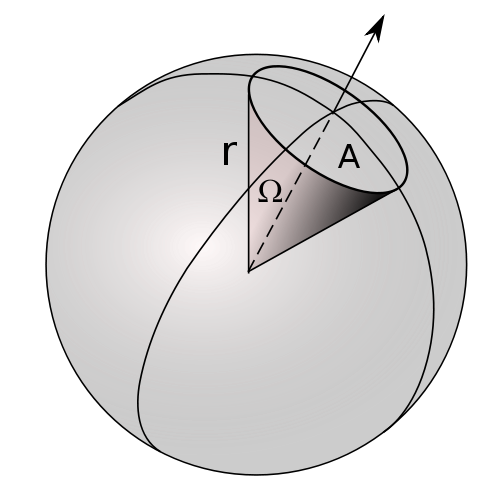
\includegraphics[scale=0.2]{Errori/solid_angle.png}
    \caption{Rappresentazione geometrica dell'angolo solido sotteso}
    \label{fig:angolo_solido}
\end{figure}
Nel nostro caso il termine $d$ è il diametro del rivelatore A , mentre $l$ è la distanza bersaglio-rivelatore A. La propagazione degli errori ha dunque prodotto la seguente espressione:
\begin{equation}
    \sigma_{\Delta\Omega} = \frac{8\pi d l}{(4l^2+d^2)^2} \sqrt{l^2 \sigma_{d}^2 + d^2 \sigma_{l}^2}
    \label{eq:err_angolo_solido}
\end{equation}
Per quanto riguarda $\sigma_d$ si è ritenuto ragionevole utilizzare l'errore strumentale del calibro ($\pm0.05\unit{\cm}$) con il quale si è misurato il diametro del rivelatore.\\La distanza bersaglio-rivelatore veniva invece misurata con il metro ed è certamente la misura con maggior contributo di errore.\\
Poichè il contributo di errore dovuto all'angolo solido è quello di maggior peso, come confermato dalla simulazione Montecarlo in sezione \ref{sezione d'urto e montecarlo}, si sono fatte alcune considerazioni in merito. Dopo alcune riflessioni si è infatti considerato che ad ogni dato angolo di misura la distanza $l$ dipende in realtá dal punto in cui interagisce il fotone con il bersaglio; motivo per cui l'errore associato é stato stimato a $\sigma_l = \pm 1 \unit{\cm}$. Questo perché considerando le ipotesi peggiori, cioé che lo scattering avvenisse sul bordo del bersaglio, la distanza $l$ effettiva si distacca in media (nelle varie configurazioni angolari) di circa $\pm 1 \unit{\cm}$ dal valore misurato di $14.4\unit{cm}$ .\\Queste riflessioni ci hanno dunque spinto ad aumentare l'errore rispetto a quello strumentale; tuttavia permettono solamente una stima qualitativa. In prospettiva sarebbe stato meglio scegliere una geometria tale da aumentare le distanze, e di conseguenza diminuire gli angoli solidi coperti, migliorando cosí l'errore percentuale sulla distanza $l$ a discapito di un minor rate di conteggi al secondo.
\subsection{Sezio d'urto e Simulazione Montecarlo}\label{sezione d'urto e montecarlo}
Per valutare l'errore associato alla misura della sezione d'urto è stata utilizzata la teoria della propagazione degli errori ottenendo la seguente fotmula:
\begin{equation}
    \sigma_{\frac{d\sigma}{d\Omega}} = \frac{M}{\Delta\Omega N_{A} \rho dx} \sqrt{\frac{N_{S}^{2}}{N_{i}^{2} \Delta\Omega^{2}} \sigma_{\Delta\Omega}^{2}+\sigma_{\frac{N_{S}}{N_{i}}}^{2}+\frac{N_{S}^{2}}{N_{i}^{2} dx^{2}}\sigma^2_{dx}}
\end{equation}
Al fine di completare l'analisi degli errori sperimentali associati alla misura della sezione d'urto dell'effetto Compton, è stata sviluppata e implementata una simulazione Montecarlo. Questo approccio è stato adottato con l'obiettivo di verificare l'accuratezza delle formule utilizzate per la propagazione degli errori e per identificare quali parametri sperimentali contribuiscano maggiormente all'incertezza complessiva della misura. Il codice utilizzato per la simulazione è reso disponibile nella repository di github\footnote{Codice consultabile al seguente link: \url{https://gitfront.io/r/MicheleScattola/GaGvFGBPX4Vm/Misure-Nucleari/tree/Compton/Montecarlo/}}. Dall'analisi dei risultati grafici ottenuti, presentati nelle Figure (\ref{fig:Simulazione_misura}) e (\ref{fig:simulazione_errori}) emerge che la propagazione degli errori è consistente con le previsioni teoriche. In particolare, è possibile constatare che il principale contributo all'incertezza nella misura della sezione d'urto è attribuibile alla misura dell'angolo solido.
\begin{figure}[H]
  \centering
  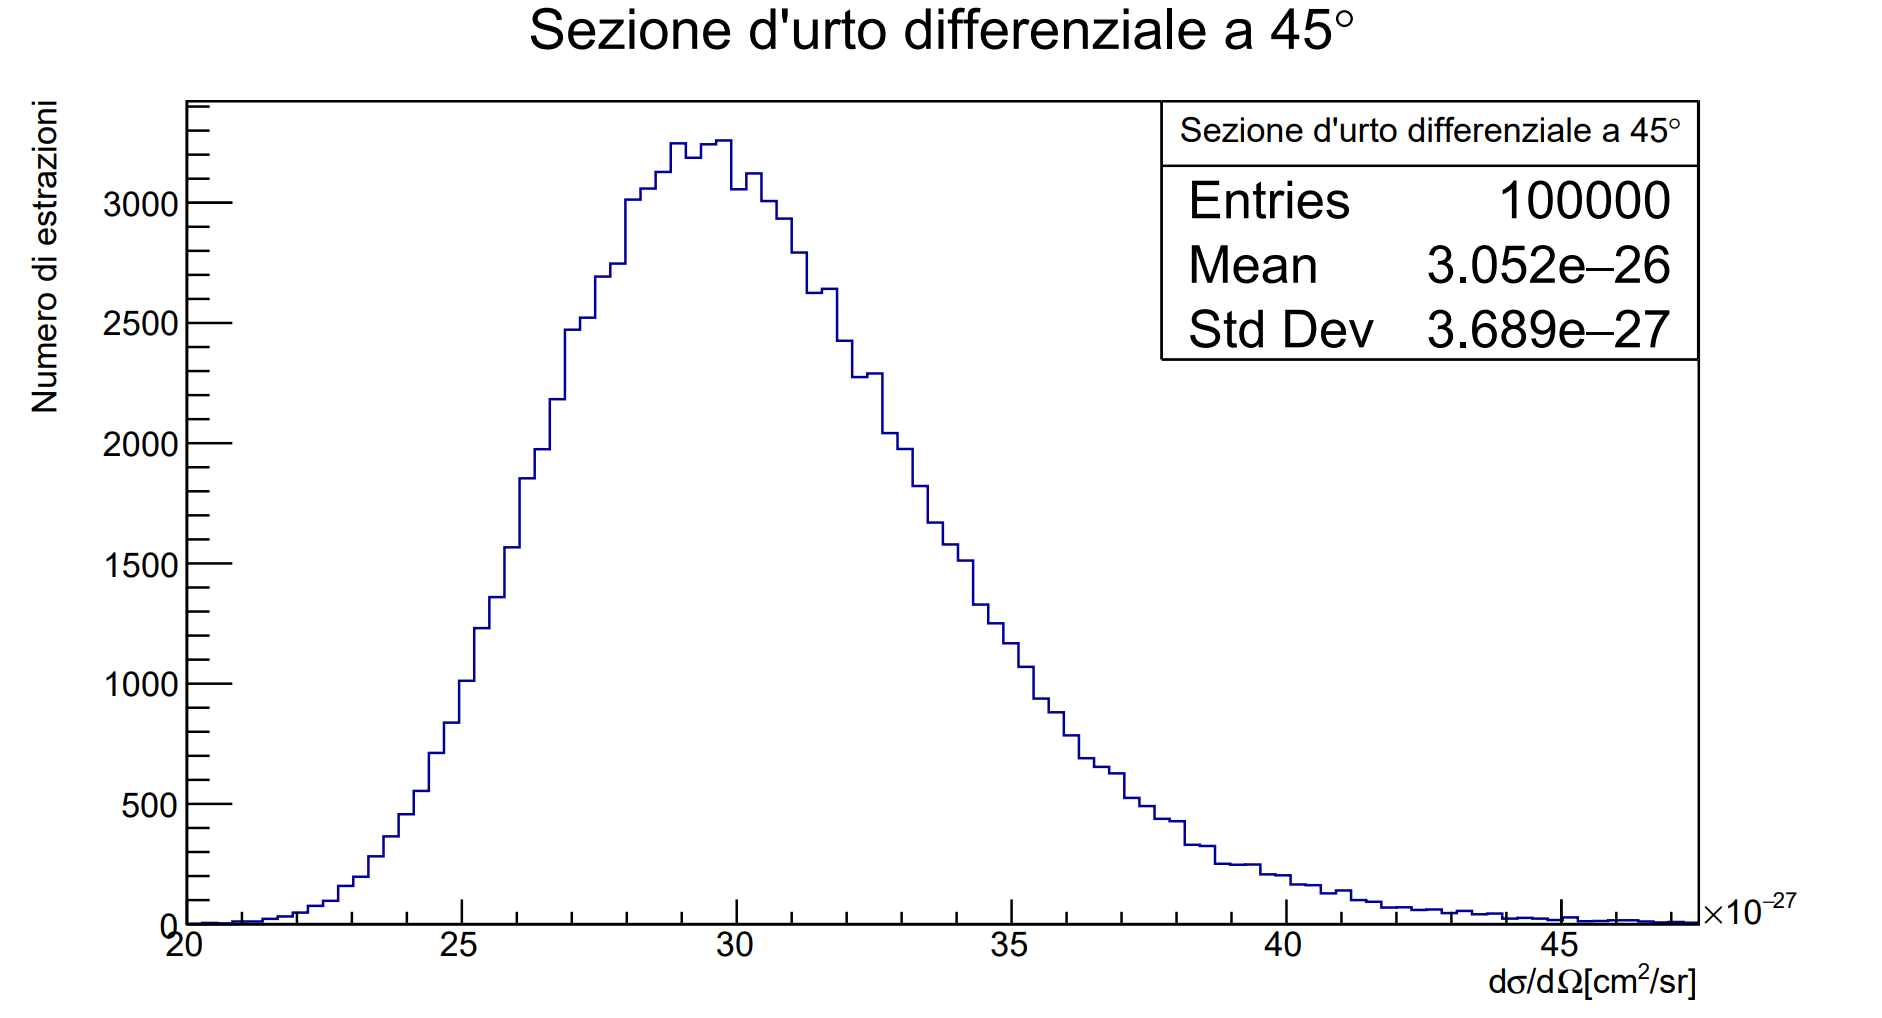
\includegraphics[scale=0.25]{Analisi Dati/SimulazioneMontecarlo_misura.png} 
  \caption{Simulazione di 100,000 misure della sezione d'urto Compton}
  \label{fig:Simulazione_misura}
\end{figure}
\begin{figure}[H]
  \centering
  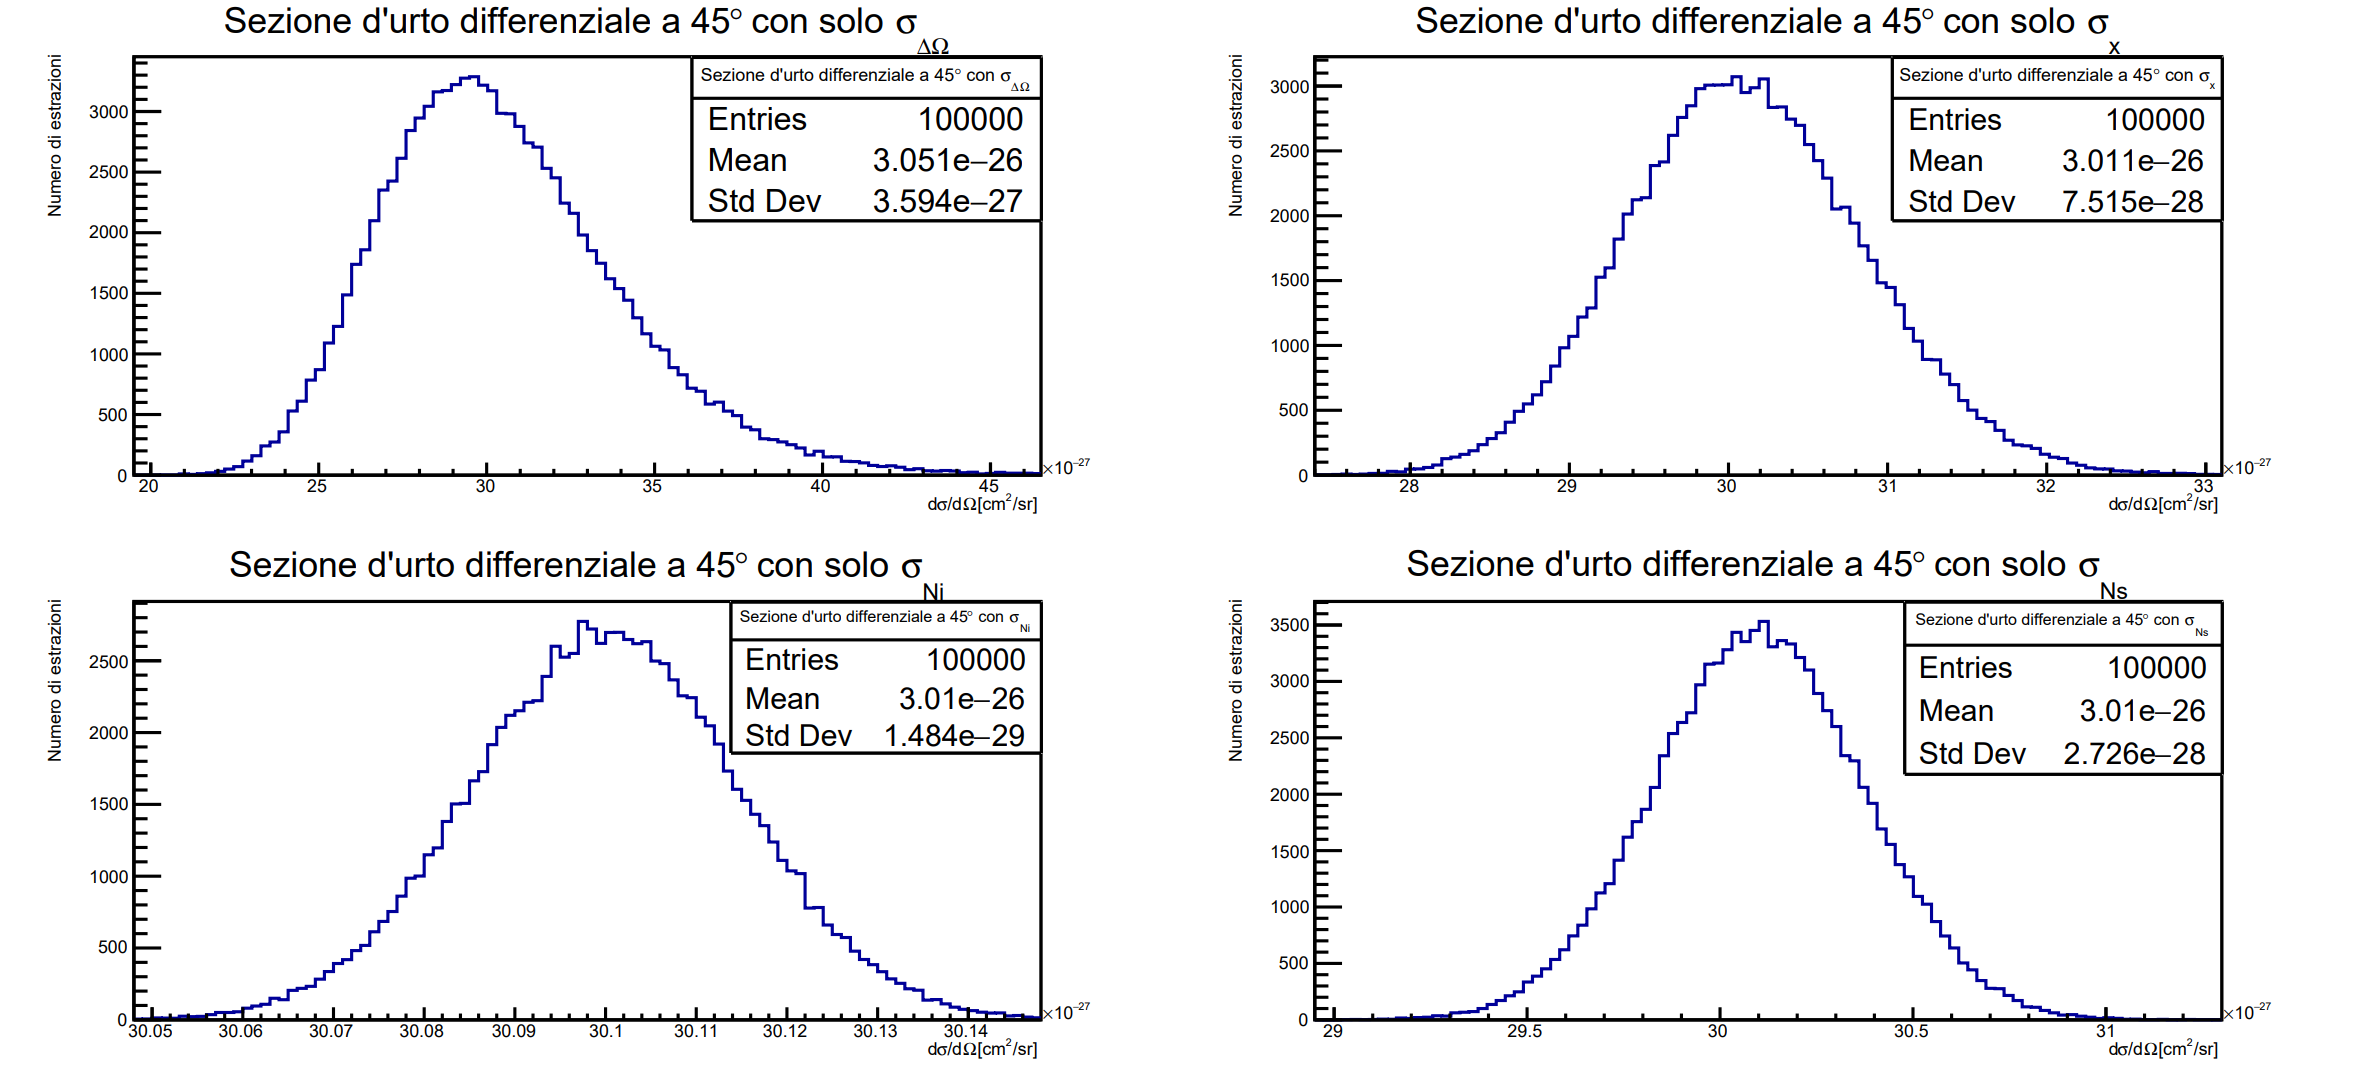
\includegraphics[scale=0.3]{Analisi Dati/SimulazioneMontecarlo_errori.png} 
  \caption{Simulazione di 100,000 misure della sezione d'urto Compton, con l'isolamento sequenziale degli errori sperimentali.}
  \label{fig:simulazione_errori}
\end{figure}

\newpage
\section{Conclusioni}
Ricapitolando, l'obbiettivo dell'esperienza è verificare la relazione che descrive l'energia di un fotone Compton in funzione dell'angolo di scattering e verificare la sezione d'urto espressa dall'equazione di Klein-Nishina. 

I risultati sperimentali ottenuti per il primo andamento e il test del $\chi^2$ dimostrano che la calibrazione e la disposizione angolare del set-up sperimentale sono state valutate correttamente e le misure effettuate sono coerenti con il modello teorico previsto. Tuttavia, per quanto riguarda la sezione d'urto sperimentale in funzione dei conteggi, il test del $\chi^2$ non è stato superato. 

Attraverso i fit parametrici si sono stimati i valori di $m_ec^2$ e del raggio dell'elettrone $r_e$ ottenendo: $m_ec^2=(523\pm12)\unit{\kilo\electronvolt}$ e $r_e=(3.01\pm0.65)\unit{fm}$. L'incertezza sul valore della massa a riposo dell'elettrone è chiaramente influenzato dalle larghezze gaussiane dei picchi misurati. La sua stima verrebbe dunque migliorata grazie ad un tempo di acquisizione maggiore, il quale aumenterebbe notevolmente la statistica. Si nota infatti che l'andamento gaussiano dei risulta maggiormente piccato all'aumentare della statistica acquisita.
La stima del raggio classico dell'elettrone risulta anch'essa confrontabile con il valore teorico ma caratterizzata da una incertezza piuttosto importante. Questo è infatti diretta conseguenza della misura sperimentale della sezione d'urto e le relative incertezze già precedentemente analizzate.

\vspace{0.5cm}
Infine, vengono qui riportate le possibili modifiche all'esperienza per migliorare la misura:
\begin{itemize}
    \item Lo studio manca di una analisi del fondo, potrebbe infatti aver influenzato il numero di conteggi osservati dal rivelatore.
    \item Come suggerito in sezione \ref{sez_err_angolo_solido} per ridurre l'errore sull'angolo solido coperto dal rivelatore sarebbe ragionevole proporre una geometria tale da aumentare le distanze coinvolte, a discapito di un rate di conteggi al secondo.
    \item Una ulteriore riflessione riguarda il bersaglio in quanto si potrebbe scegliere uno spessore particolarmente ridotto, rendendo così maggiormente confrontabili la lunghezza percorsa al suo interno dal fotone prima di interagire e lo spessore $dx$ presente nella sezione d'urto sperimentale.
\end{itemize}

\newpage
\section{Appendice}

\subsection{Spettri a vari angoli}\label{appendice_spettri}
\begin{figure}[htbp]
    \centering
    % First row
    \begin{subfigure}[b]{0.45\textwidth}
        \centering
        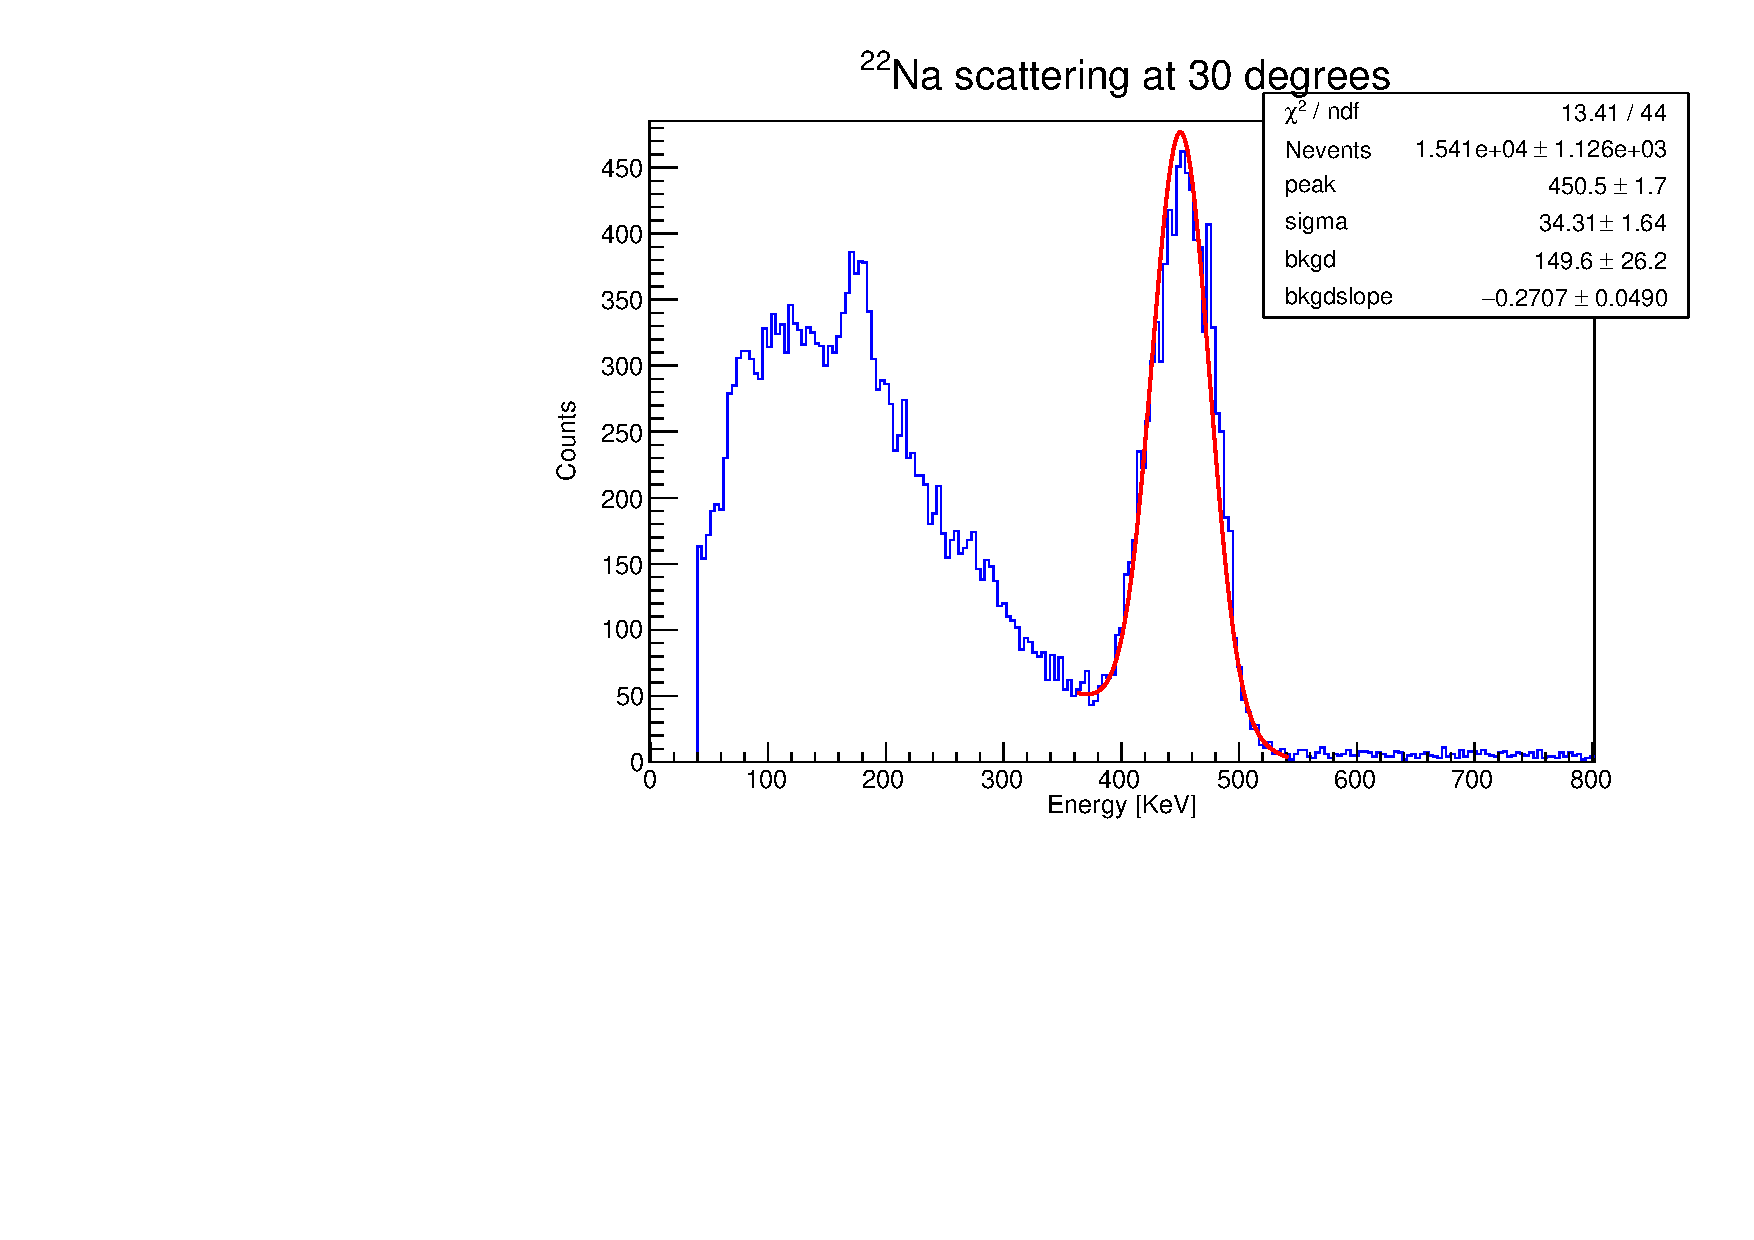
\includegraphics[width=\textwidth]{Appendice/30_deg_spectrum.pdf}
    \end{subfigure}
    \hfill
    \begin{subfigure}[b]{0.45\textwidth}
        \centering
        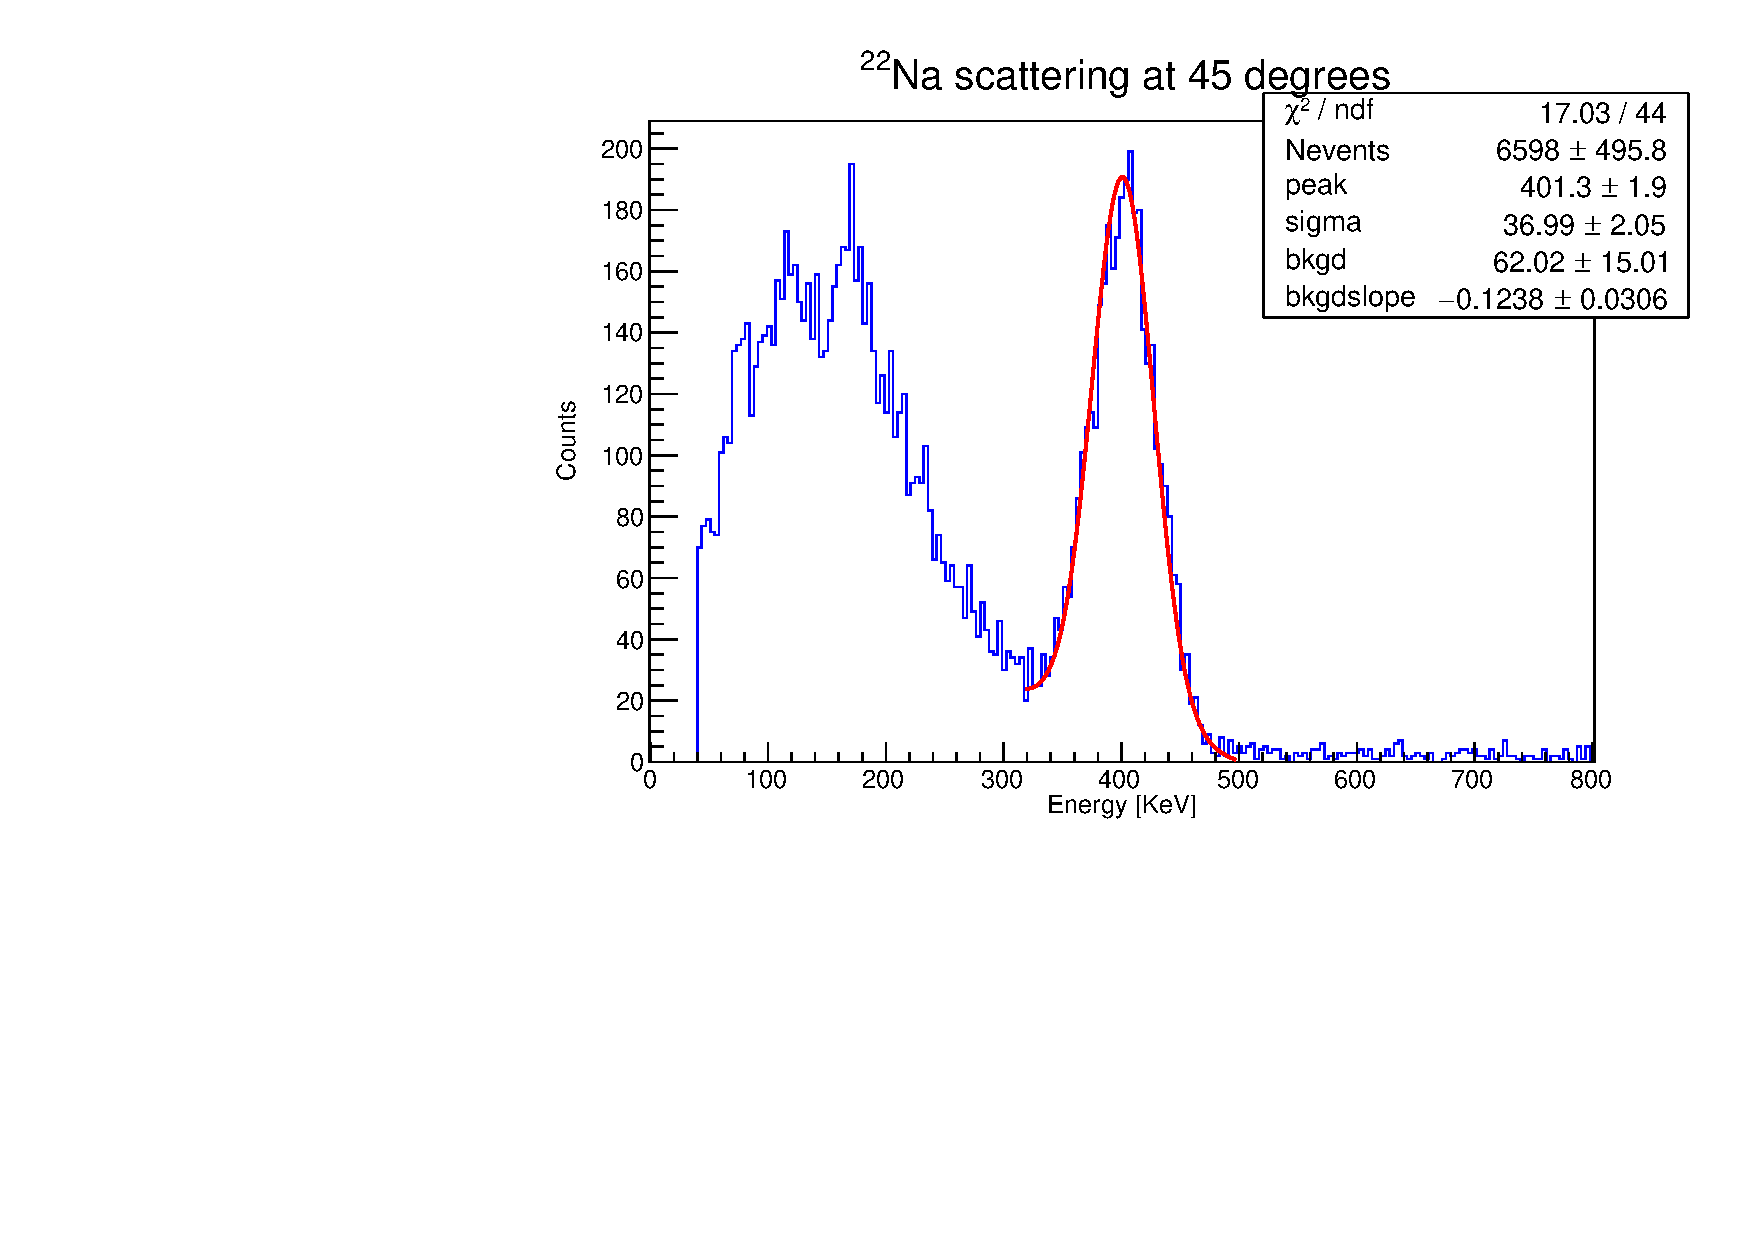
\includegraphics[width=\textwidth]{Appendice/45_deg_spectrum.pdf}
    \end{subfigure}
    
    \vspace{0.5cm} % Add vertical space between rows

    % Second row
    \begin{subfigure}[b]{0.45\textwidth}
        \centering
        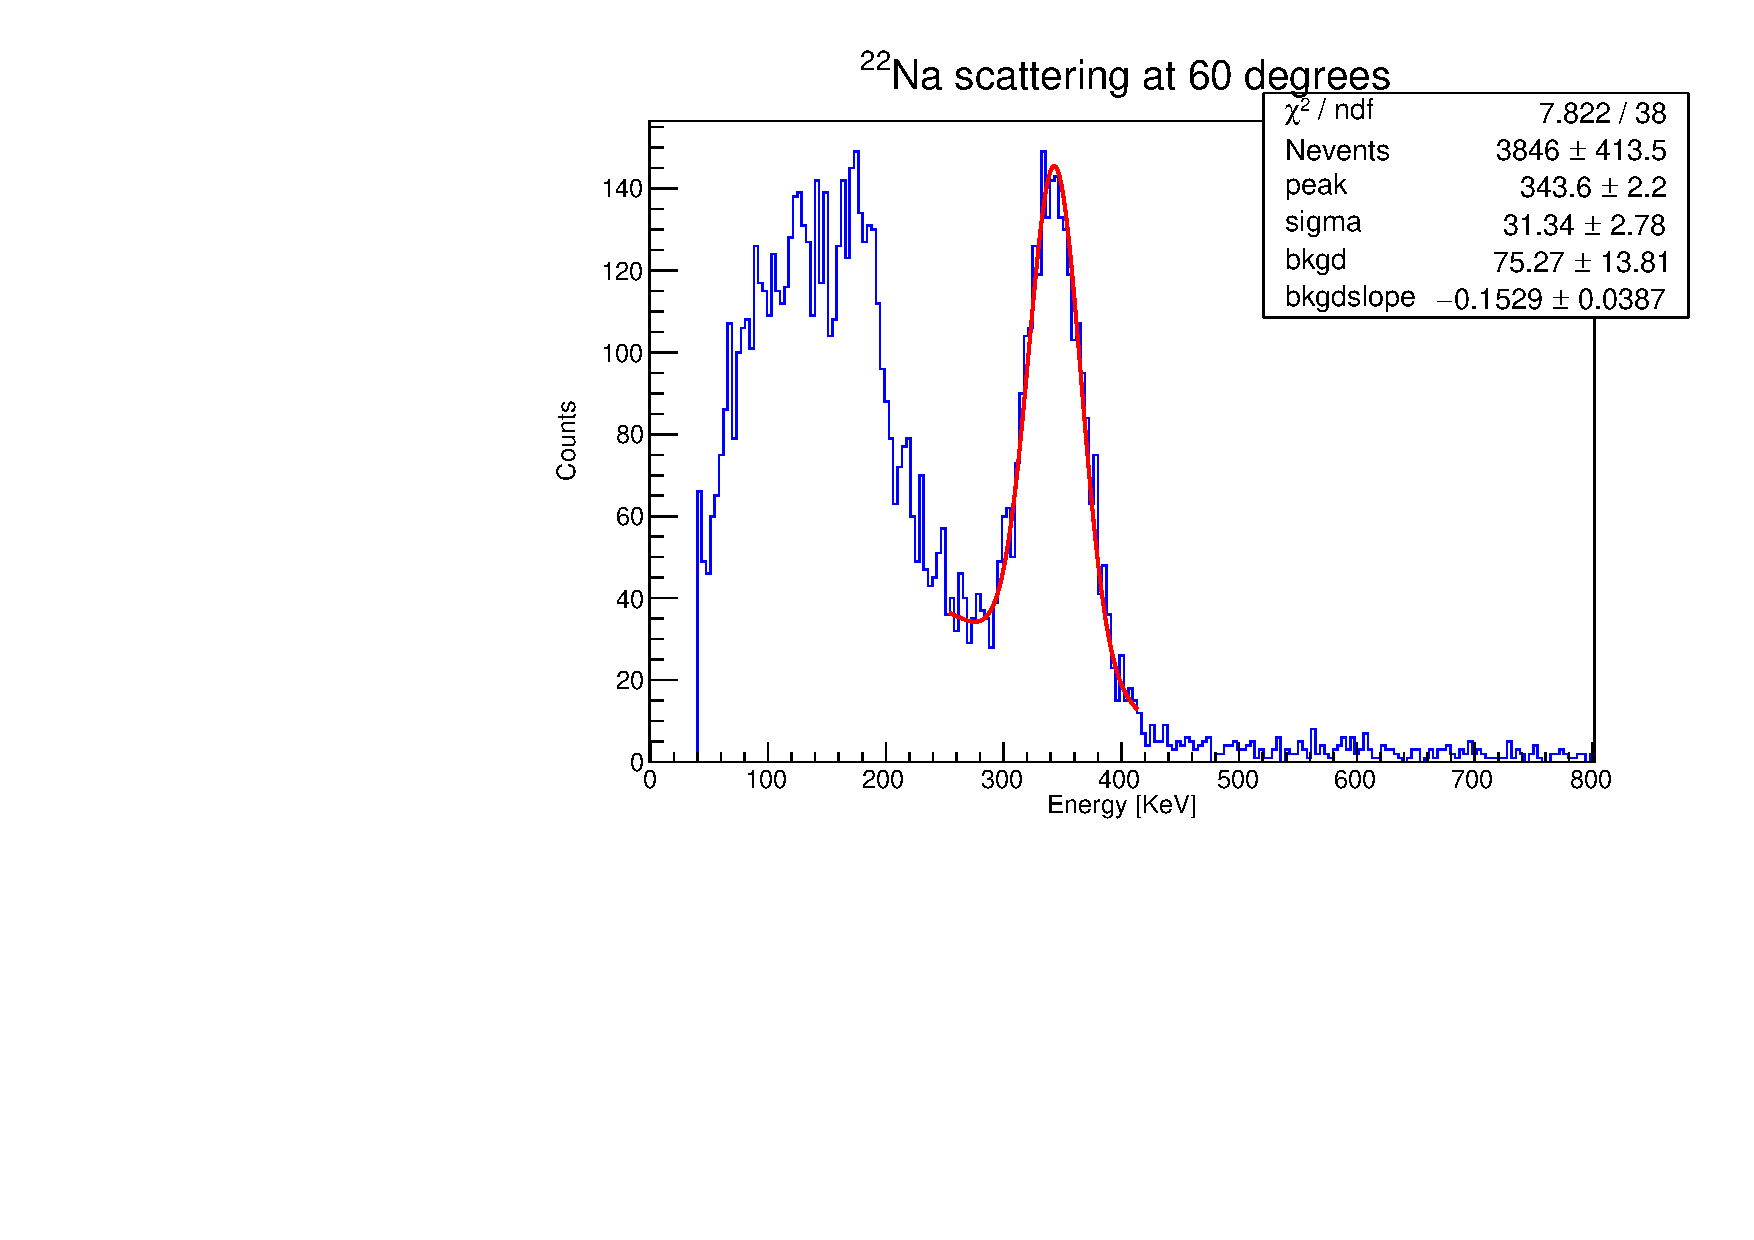
\includegraphics[width=\textwidth]{Appendice/60_deg_spectrum.pdf}
    \end{subfigure}
    \hfill
    \begin{subfigure}[b]{0.45\textwidth}
        \centering
        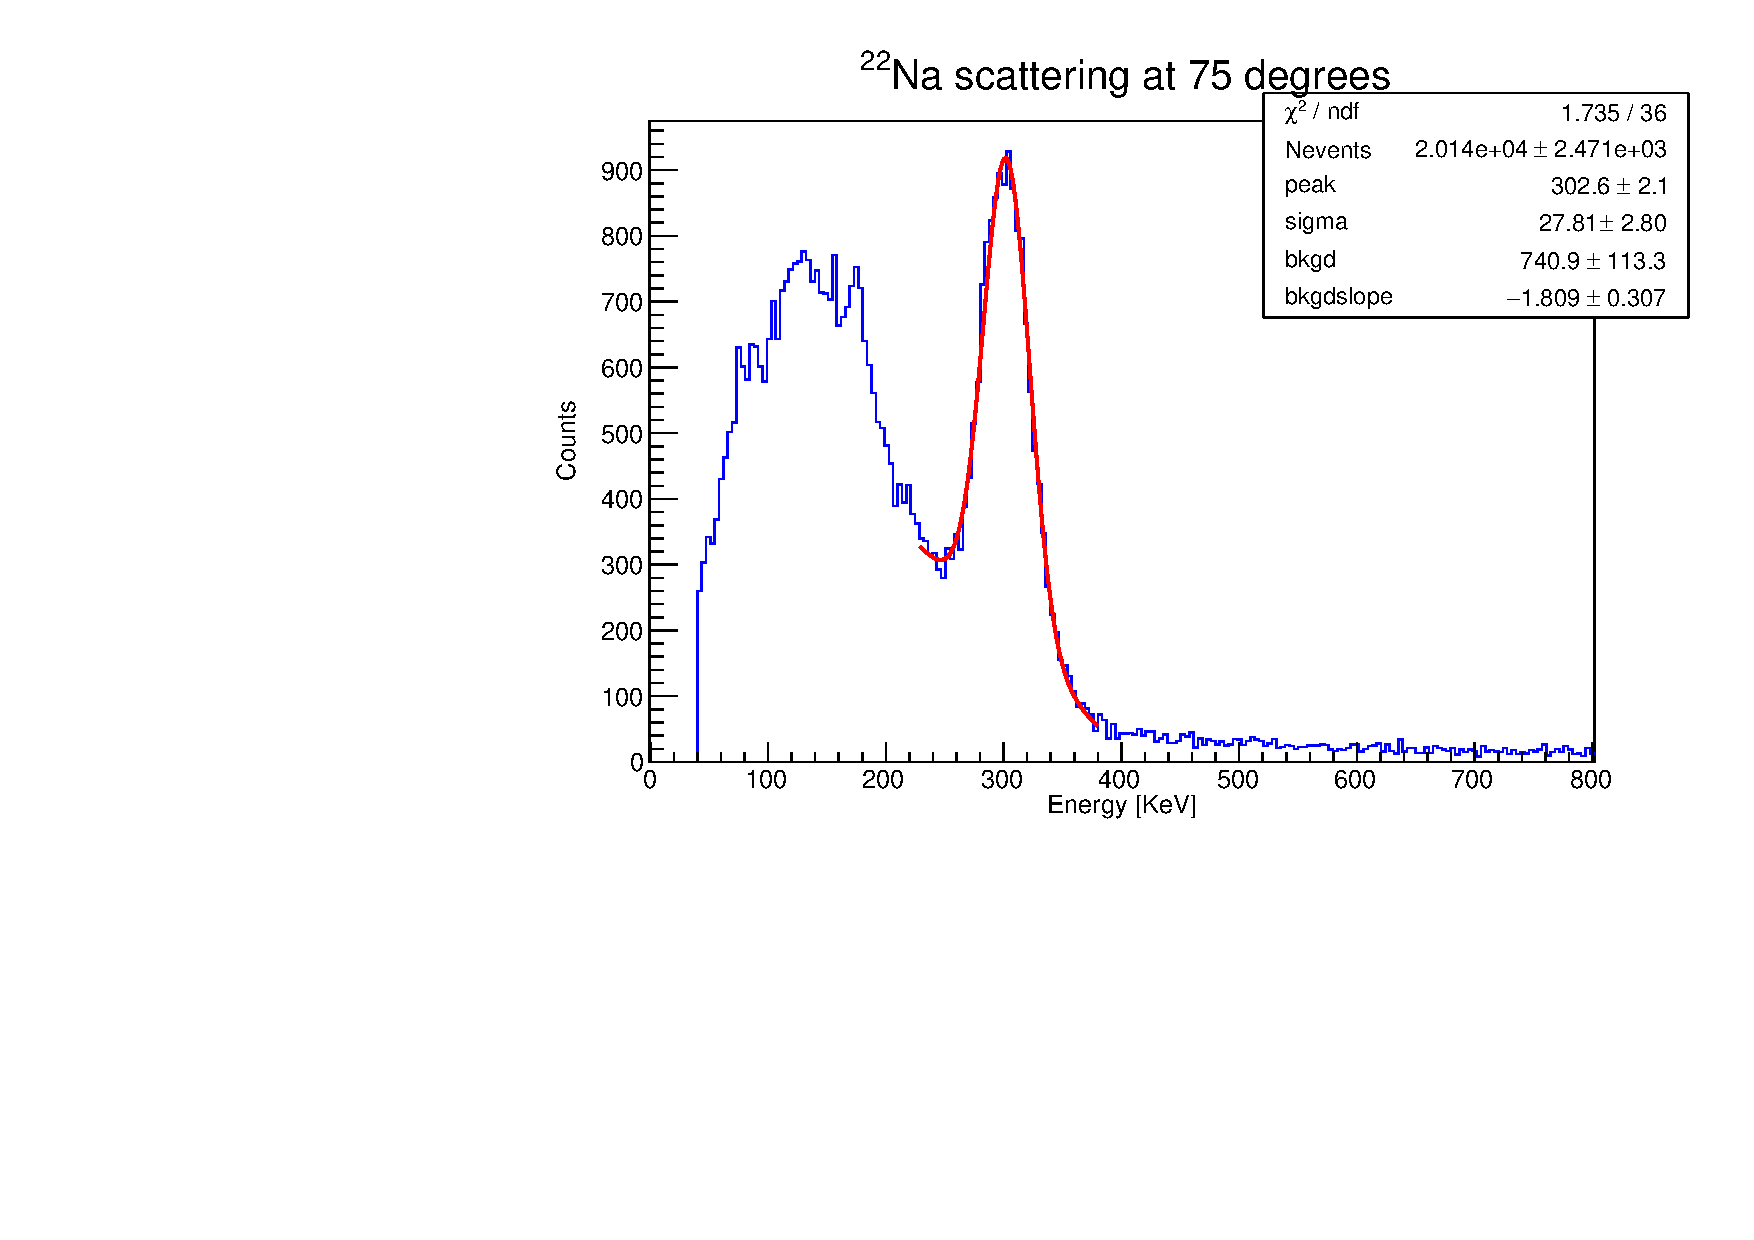
\includegraphics[width=\textwidth]{Appendice/75_deg_spectrum.pdf}
    \end{subfigure}
    
    \vspace{0.5cm} % Add vertical space between rows

    % Third row
    \begin{subfigure}[b]{0.45\textwidth}
        \centering
        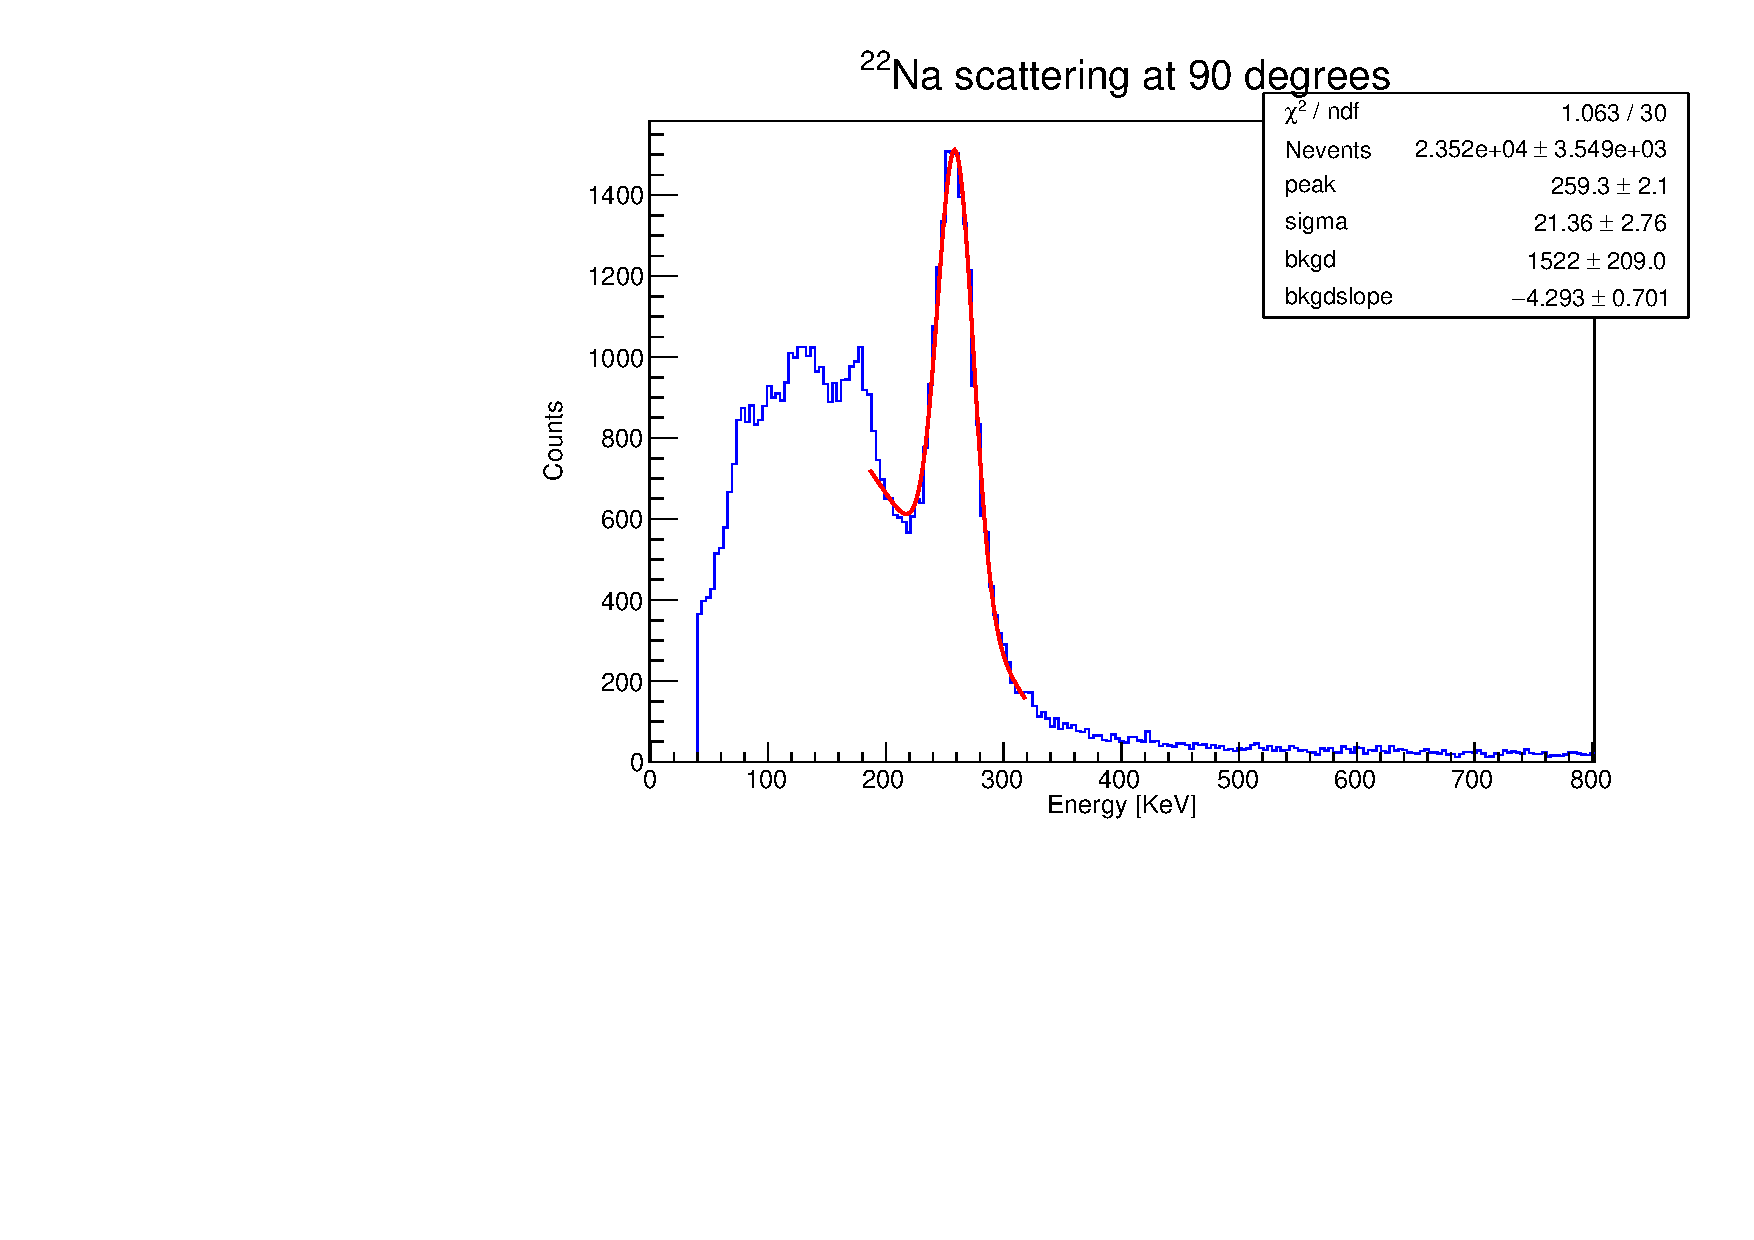
\includegraphics[width=\textwidth]{Appendice/90_deg_spectrum.pdf}
    \end{subfigure}
    \hfill
    \begin{subfigure}[b]{0.45\textwidth}
        \centering
        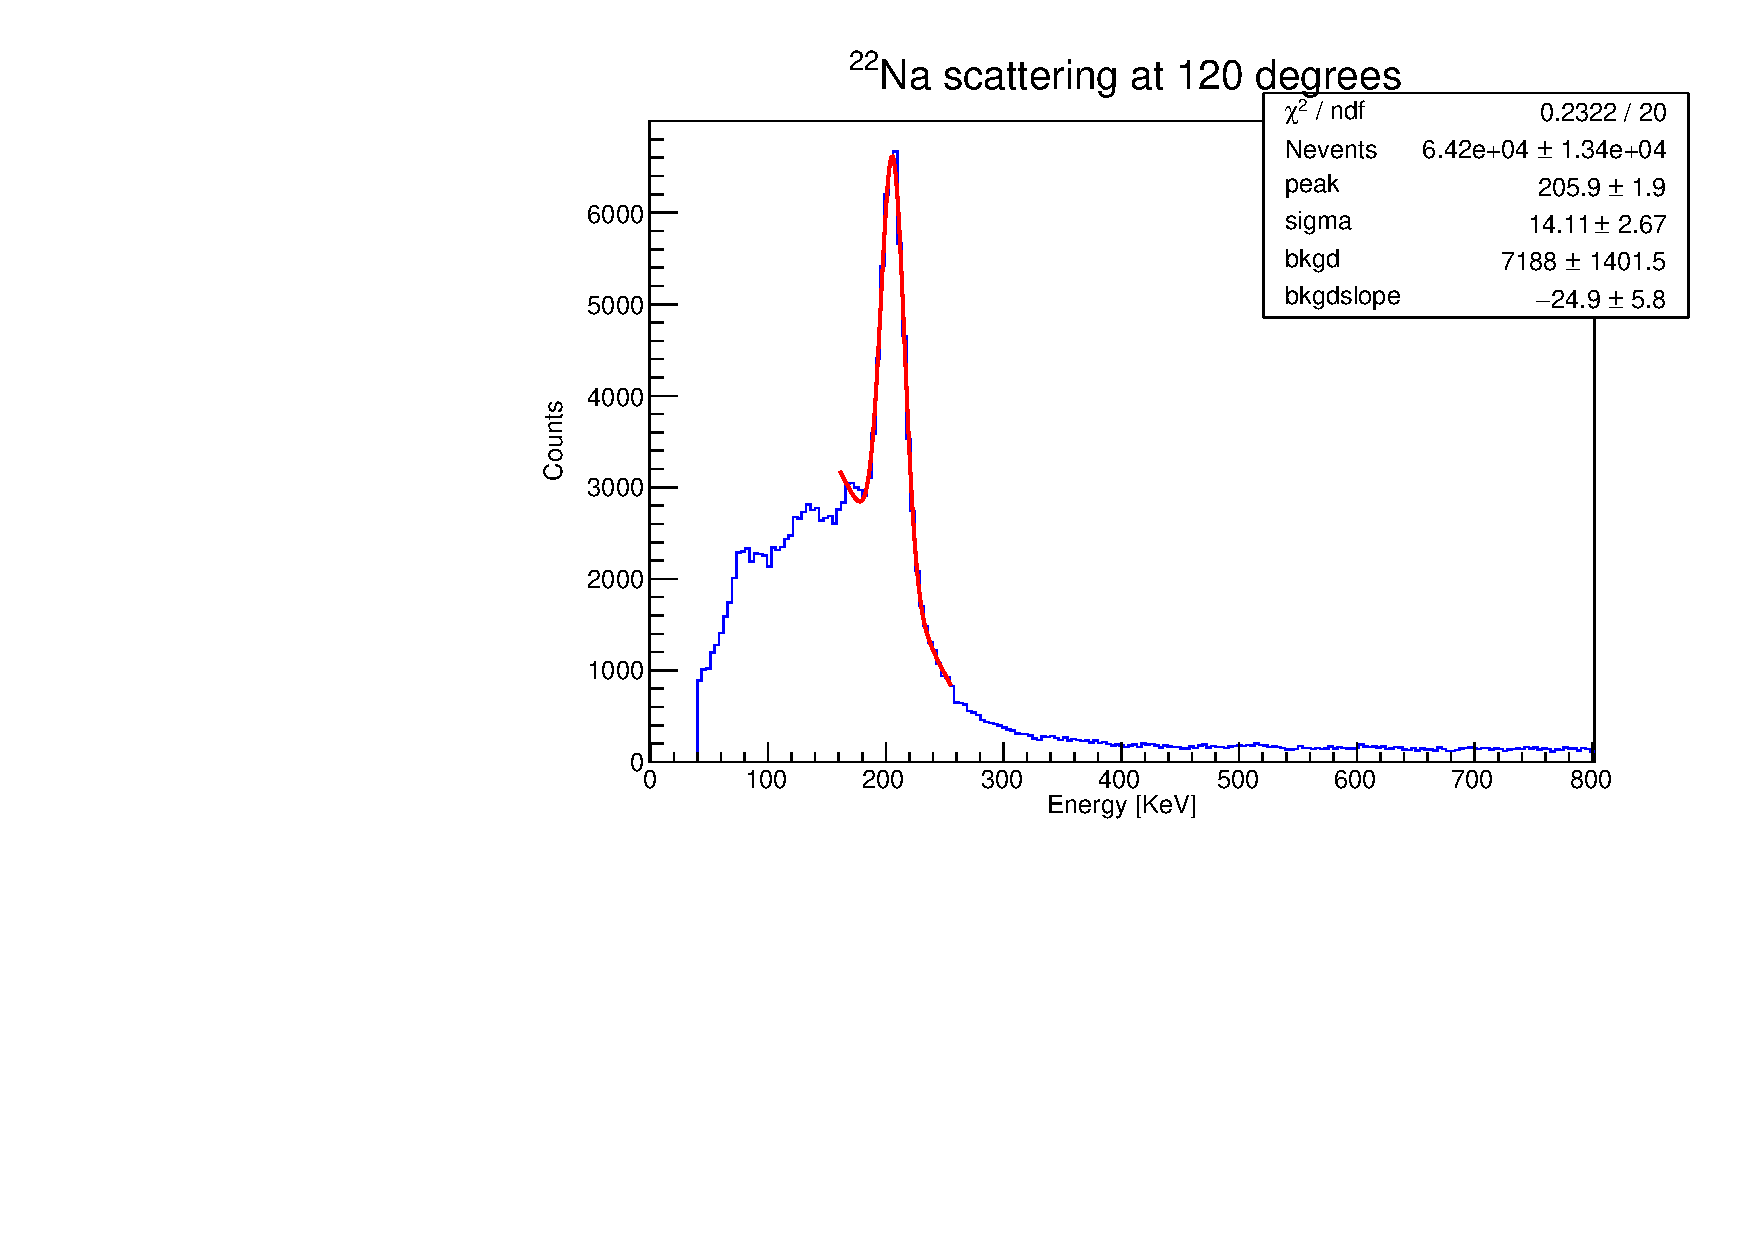
\includegraphics[width=\textwidth]{Appendice/120_deg_spectrum.pdf}
    \end{subfigure}
    
    \caption{Spettri acquisiti ai vari angoli}
    \label{fig:appendice_spettri}
\end{figure}

%\subsection{Errore sezione d'urto energetica}\label{appendice_errore_sezione_energie}
%L'errore calcolato per progazione della formula di Klein-Nishina risulta il seguente:
%\begin{equation}
   % \sigma_{\frac{d\sigma}{d\theta}} = r_e^2 \sqrt{\left( \frac{9}{4} k_1 + \frac{1}{4} + k_1^2\sin{\theta}^4+\frac{3}{2} k_1^2 -3k_1^3 \sin{\theta}^2-k_1\sin{\theta}^2 \right)\sigma_{k_1}^2 + \left(k_1^4 \sin{\theta}^2 \cos{\theta}^2\right) \sigma_{\theta}^2}
    \label{err_klein_nishina}
%\end{equation}
%dove $k_1 = \frac{E_1}{m_e c^2}$
\subsection{Dati grezzi}
\begin{table}[H]
    \centering
    \begin{tabular}{|c|c|c|c|c|}
    \hline
       Sorgente & $E_{teorica} [\unit{\kilo\electronvolt}]$ & $\sigma_{teorica}$ & ADC Channel & $\sigma_{ch}$\\
       \hline
       \hline
       $\ch{^{22}Na}$ & $511.000$ & $0.001$ & $1374.00$ & $45.87$\\
        \hline
       $\ch{^{22}Ne}$ & $1274.537$ & $0.01$ & $3439.23$ & $56.42$\\
       \hline
       $\ch{^{137}Cs}$ & $661.657$ & $0.003$ & $1783.36$ & $52.02$\\
       \hline
    \end{tabular}
    \caption{Misure dagli spettri di calibrazione ADC.}
    \label{tab:ADC}
\end{table}
\begin{table}[H]
    \centering
    \begin{tabular}{|c|c|c|c|c|c|}
    \hline
       Angolo & $E_{teorica} [\unit{\kilo\electronvolt}]$ & $E_{misurata}[\unit{\kilo\electronvolt}]$ & $\sigma$ & $N_{picco}$ & $\sigma/\sqrt{N}$\\
       \hline
       \hline
       $0^\circ$ & $511.000$ & $507.831$ & $15.97$ & $23800$ & $0.104$ \\
        \hline
       $30^\circ$ & $450.627$ & $450.451$ & $34.31$ & $8919$ & $0.363$ \\
       \hline
       $45^\circ$ & $395.238$ & $401.287$ & $36.99$ & $3790$ & $0.601$ \\
       \hline
       $60^\circ$ & $340.667$ & $343.667$ & $31.34$ & $3002$ & $0.572$ \\
       \hline
       $75^\circ$ & $293.479$ & $302.629$ & $27.81$ & $17986$ & $0.207$ \\
       \hline
       $90^\circ$ & $255.500$ & $259.277$ & $21.37$ & $27831$ & $0.128$ \\
       \hline
       $120^\circ$ & $204.400$ & $205.918$ & $14.11$ & $84629$ & $0.048$ \\
       \hline
    \end{tabular}
    \caption{Misure dagli spettri ai vari angoli.}
    \label{tab:appendice_spettri}
\end{table}
\begin{table}[H]
    \centering
    \begin{tabular}{|c|c|c|c|c|}
    \hline
       angoli& $N_i$ & $N_S$ & $\frac{N_s}{N_i}$ & $\sigma_{\frac{N_s}{N_i}}$\\
       \hline
       \hline
       $30^\circ$ & $7500140$ & $28398$ & $0.00379$ & $0.00002$\\
        \hline
       $45^\circ$ & $3882437$ & $11786$ & $0.00304$ & $0.00003$\\
       \hline
       $60^\circ$ & $3590958$ & $8661$ & $0.00241$ & $0.00003$\\
       \hline
       $90^\circ$ & $7676854$ & $14245$ & $0.00186$ & $0.00002$\\
       \hline
    \end{tabular}
    \caption{In questa tabella sono riportati i dati ricavati dalle misure in laboratorio.}
    \label{tabella dati}
\end{table}
\begin{table}[H]
    \centering
    \begin{tabular}{|c|c|c|c|}
    \hline
       $\Delta \Omega\,[\unit{sr}]$& $\sigma_{\Delta \Omega}\,[\unit{sr}]$ & $dx\,[\unit{cm}]$ & $\sigma_{dx}\,[\unit{cm}]$ \\
       \hline
       \hline
       $0.06098$ & $0.00844$ & $2.02$ & $0.05$\\
       \hline
    \end{tabular}
    \caption{In questa tabella sono presenti i dati utilizzati per calcolare la sezione d'urto,}
    \label{tabella}
\end{table}
\end{document}
